%% Influence Miner for Bitcoin - full-length version (ACM acmart format). Generated by build/assemble_bitcoin.py.
%% Populated with the full run of Influence Miner (heuristic-v2, run 3) over the
%% DeMaP Miner Python corpus, 12 September 2026.
%% Compile with:  pdflatex influence-miner-acm-results.tex  (acmart.cls in the same folder)
%% For review submission: \documentclass[manuscript,screen,review,anonymous]{acmart}

\documentclass[sigconf,screen]{acmart}

\AtBeginDocument{%
  \providecommand\BibTeX{{Bib\TeX}}}

\usepackage{booktabs}
\usepackage{pgfplots}
\usepackage{tikz}
\pgfplotsset{compat=1.18}
\usetikzlibrary{shapes.geometric,arrows.meta,positioning}

%% Draft metadata. Replace with the official ACM rights block after acceptance.
\setcopyright{none}
\copyrightyear{2026}
\acmYear{2026}
\acmDOI{}
\acmConference[Draft]{Draft manuscript prepared using the ACM acmart template}{September 2026}{New Zealand}
\acmISBN{}
\settopmatter{printacmref=false}

\begin{document}

\title[Influence Miner for Bitcoin]{Influence Miner for Bitcoin: How Influence Is Exercised in Bitcoin Improvement Proposal Discussions, 2011--2026}

\author{Pankaj Sharma}
\affiliation{%
  \institution{Universal College of Learning (UCOL)}
  \city{Palmerston North}
  \country{New Zealand}}

\renewcommand{\shortauthors}{Sharma}

\begin{abstract}
Bitcoin changes its rules without anyone being in charge of them. Proposals are written as Bitcoin Improvement Proposals (BIPs), argued on the bitcoin-dev mailing list, and adopted or not by the maintainers, miners, wallets, exchanges and node operators who decide what to run. This paper applies Influence Miner, a tool and taxonomy for mining sentence-level influence signals from open source decision-making discussions, to the complete public record of those arguments: every bitcoin-dev message from June 2011 to September 2026 (24,391 messages), linked to the 205 BIPs they discuss, with the status history of every BIP taken from the \texttt{bitcoin/bips} repository and roles derived from the reference implementation's history. Influence Miner classifies each signal into thirteen base mechanisms and seven controversial ones---unilateral decision, corporate interest, gatekeeping, exit threat, incivility, backchannel and procedural control---and attaches direction, scope, target, role, outcome and timing. The 62,791 candidate sentences show a profile unlike Python's, on which the tool was developed: ecosystem (34\%), operational (22\%), security (17\%) and economic (15\%) arguments dominate, functional arguments about whether a design solves its problem are rare (8\%), and authority is invoked in 2.5\% of sentences; 58\% of the signals come from community members and 1\% from the lead maintainer, who vanishes from the record after 2015. The block-size war of 2015--2017 was argued as a compatibility question and was, on this measure, less contested than the early or the post-2022 years; security and economic argument have risen monotonically to the present; rejected BIPs attract compatibility, economic and authority signals while accepted ones move to attacks and implementation; and stance volume predicts outcomes no better than chance. The repository's status changes record deployments, not decisions, so the decision-window peak found in Python does not exist in Bitcoin. Controversial mechanisms mark 3.9\% of sentences, led by incivility and backchannel references, concentrated in the earliest years and in the post-lead era. Measured on the same instrument, Bitcoin and Python differ in what they argue about and who argues, and agree in how explicitly they argue. The contributions are a reproducible Bitcoin corpus, the first sentence-level influence profile of Bitcoin's proposal discussions, the cross-project comparison the taxonomy was designed for, and a year-by-year timeline of the influence acts the tool nominates from the corpus itself.
\end{abstract}


\begin{CCSXML}
<ccs2012>
 <concept>
  <concept_id>10011007.10011006.10011050</concept_id>
  <concept_desc>Software and its engineering~Open source model</concept_desc>
  <concept_significance>500</concept_significance>
 </concept>
 <concept>
  <concept_id>10003120.10003121</concept_id>
  <concept_desc>Human-centered computing~Collaborative and social computing</concept_desc>
  <concept_significance>300</concept_significance>
 </concept>
 <concept>
  <concept_id>10002951.10003260.10003261</concept_id>
  <concept_desc>Information systems~Data mining</concept_desc>
  <concept_significance>300</concept_significance>
 </concept>
</ccs2012>
\end{CCSXML}

\ccsdesc[500]{Software and its engineering~Open source model}
\ccsdesc[300]{Human-centered computing~Collaborative and social computing}
\ccsdesc[300]{Information systems~Data mining}

\keywords{open source software, decision-making, influence mining, governance, Python Enhancement Proposals, Bitcoin Improvement Proposals, mailing lists, software repository mining}

\maketitle

\section{Introduction}

Bitcoin is governed by nobody and changed by somebody. Its consensus rules are enforced by every node that runs the software, so no person or body can alter them by decree; yet the rules do change---P2SH in 2012, CHECKLOCKTIMEVERIFY in 2015, Segregated Witness in 2017, Taproot in 2021---and each change was proposed, argued, revised, activated or abandoned by identifiable people writing on a public mailing list. The Bitcoin Improvement Proposal (BIP) process \cite{bip2} is the paper trail of those changes: a BIP is a design document that describes a change to the protocol, the peer-to-peer network, wallets or the process itself; it is discussed on the bitcoin-dev list, assigned a number by a BIP editor, and moves through a small set of statuses (Draft, Proposed, Final, Active, Deferred, Rejected, Withdrawn, Replaced, Obsolete; since the 2025 revision of the process, Draft, Deployed, Complete and Closed \cite{bip2}). Publication of a BIP does not mean that the community has accepted it \cite{bitcoinbips}; whether a proposal is adopted depends on discussion, on implementations, on the choices of miners, node operators, wallets and exchanges, and---for consensus changes---on an activation mechanism that has itself been the subject of some of the community's bitterest disputes \cite{bip8, bip148}.

This makes Bitcoin an unusually good place to study influence. In a project such as Python, a decision has a formal owner: the BDFL, a delegate, or the Steering Council can pronounce a proposal accepted \cite{pep1, pep13}. Bitcoin has no such office. It has maintainers of the reference implementation with merge access, a lead maintainer until January 2022, editors who administer the BIP repository, proposal authors, companies that employ most of the active developers, miners whose signalling activates soft forks, and a large community of node operators, wallet developers and users who can refuse to run new code. Prior work has characterised this arrangement as ``invisible politics'' \cite{defilippi2016}, as ``senatorial'' governance by competing bureaucratic parties \cite{parkin2019}, as a fiduciary relationship between developers and users \cite{walch2019}, and, quantitatively, as a system in which a handful of people account for most of the discussion \cite{azouvi2018}. What such accounts leave open is \emph{how} influence is exercised in the discussions themselves: with which arguments, by whom, at what point of a proposal's life, and through which of the contested forms---decisions by fiat, corporate stakes, gatekeeping, threats to fork, incivility, off-list agreements, procedural control---that the block-size war of 2015--2017 made visible to everyone \cite{bier2021}.

This paper applies Influence Miner, the tool and taxonomy introduced for Python \cite{influenceMinerPython}, to the complete public record of Bitcoin's proposal discussions: every message on the bitcoin-dev mailing list from its creation in June 2011 to September 2026, linked to the BIPs it discusses, together with the status history of every BIP from the \texttt{bitcoin/bips} repository and role rosters derived from the \texttt{bitcoin/bitcoin} repository. Influence Miner classifies sentence-level influence signals into thirteen base mechanisms (strategic, operational, functional, tactical, authority, compatibility, security, standards, ecosystem, economic, organizational, coalition and user demand) and seven controversial ones (unilateral, corporate interest, gatekeeping, exit threat, incivility, backchannel and procedural control), and attaches to each signal a direction, a scope, a target, the author's role, the proposal's outcome and the signal's timing relative to the decision. The taxonomy was designed with Bitcoin in mind---its cue lists already carried soft forks, miners, wallets, exchanges, fee markets and consensus failures---and this paper is its first test on the community those cues were written for.

The paper makes four contributions. First, it delivers the Bitcoin corpus itself: a reproducible pipeline that turns the public-inbox archive of bitcoin-dev, the BIP repository's history and the reference implementation's commit history into the same relational form that the DeMaP Miner family of tools uses for Python, with 24,391 messages, 205 BIPs and role labels for every message. Second, it reports the first sentence-level influence profile of Bitcoin's proposal discussions and answers six research questions about mechanisms, actors, eras, outcomes, the overlap with preference signals and controversial influence. Third, it compares Bitcoin with Python on the same instrument and finds the differences the taxonomy predicted---more ecosystem, economic and security influence, weaker internal authority, more exit and coalition pressure---together with differences it did not predict. Fourth, it uses the tool to nominate the landmark influence acts of each year of Bitcoin's history and sets them against the events the community itself remembers.

As with the Python study, the labels are produced by transparent cue rules that have not yet been validated against a gold standard; the results are a baseline and a demonstration that the pipeline transfers, not final measurements of influence in Bitcoin.

\section{Background and Motivation}
\label{sec:background}

\subsection{Bitcoin's Decision-Making Arrangements}

Bitcoin's founder left the project in December 2010, handing the repository to Gavin Andresen, who acted as lead maintainer until April 2014 and was succeeded by Wladimir van der Laan until January 2022; since then Bitcoin Core has had several maintainers with merge access and no lead \cite{bier2021}. Maintainers merge code; they do not decide consensus rules. A consensus change is a BIP that must be implemented, released and \emph{activated}: for soft forks, by miners signalling readiness (BIP 9), by height-based lock-in (BIP 8), or by users running software that enforces the new rules on a flag day (BIP 148) \cite{bip8, bip148}. Node operators, wallets, exchanges and miners can therefore veto or force a change by what they run, which is why so much of the argument on bitcoin-dev is about what the ecosystem will accept rather than about what the maintainers want. The BIP process itself is administered by editors---Amir Taaki, then Gregory Maxwell, then Luke Dashjr from 2016 to 2026, joined by Kalle Alm in 2021 and replaced by a panel of five in 2024---whose job is to assign numbers and merge documents, not to judge proposals \cite{bip2}; the 2025 revision of the process (BIP 3) restated this and relabelled the status vocabulary.

Three episodes shaped the community's understanding of its own governance and recur throughout this paper. The \emph{block-size war} of 2015--2017 began with BIP 101 and the Bitcoin XT client, continued through Bitcoin Classic and Unlimited, the Hong Kong and New York agreements between companies and miners, and ended with the user-activated soft fork (BIP 148), the Bitcoin Cash split and the activation of Segregated Witness in August 2017; it was fought largely on bitcoin-dev and established that neither maintainers nor miners nor companies could impose a rule change on unwilling users \cite{bier2021, defilippi2016}. The \emph{Taproot activation} debate of 2021 replayed the activation question (BIP 8 with mandatory lock-in versus BIP 9-style ``Speedy Trial'') without the acrimony, and Taproot activated in November 2021. The \emph{post-lead era} since 2022 has seen contested proposals for covenants (BIP 119, BIP 347), drivechains (BIP 300/301), the relay policy for inscriptions and \texttt{OP\_RETURN}, and the BIP editorship itself, and the list moved from the Linux Foundation to Google Groups in February 2024.

\subsection{How Bitcoin and Open Source Projects Are Influenced}

The literature on influence in open source development reviewed in the Python study \cite{influenceMinerPython}---core/periphery structure \cite{mockus2002, crowston2005}, status \cite{stewart2005}, lateral authority \cite{dahlander2011}, governance modes \cite{omahony2007, markus2007, shaikh2017}, the evaluation of contributions \cite{tsay2014, alami2020}, firms \cite{schaarschmidt2015, zhang2022}, conflict and incivility \cite{filippova2016, ferreira2021, miller2022}, exit and forks \cite{hirschman1970, robles2012}---applies to Bitcoin with two twists. First, the fork is not a last resort but a constitutional instrument: Bitcoin's rules are whatever the economically dominant chain enforces, so the threat to fork, the counter-threat to reject a fork, and the coalition-building that precedes both are the ordinary currency of its hardest decisions \cite{bier2021, bohme2015}. Second, the ``users'' are not passive: mining pools, exchanges, wallet vendors and node operators are organised actors whose choices decide activation, and whose representatives write on the list. Bitcoin-specific studies have quantified the concentration of code and discussion in a few hands \cite{azouvi2018} and of mining and network resources \cite{gencer2018, gervais2014}, described the political structure as technocratic and largely invisible to users \cite{defilippi2016}, as senatorial competition among bureaucratic parties \cite{parkin2019}, and as an off-chain governance layer that the code cannot replace \cite{reijers2021}; the earlier Bitcoin work of the DeMaP Miner group identified the ``influencers'' of three rule changes by network centrality and, from the mailing list, IRC minutes and podcasts, described five tactics they used---political neutrality, shepherding the community, a participative approach, sticking to the laid plan and developing reciprocal relationships---built on the lateral-influence tactics of Ngwenyama and Nielsen \cite{thapa2021bitcoin, ngwenyama2014}; Section~\ref{sec:icis} returns to those three BIPs and maps the tactics onto the mechanisms. None of this work classifies the arguments at the sentence level or follows them across the whole history of the list; that is what Influence Miner adds.

\subsection{The DeMaP Miner Line}

This study is the Bitcoin arm of the DeMaP Miner research agenda, which has mined decision-making processes \cite{sharma2022demap}, rationales \cite{sharma2024rationale}, preferences and, most recently, influence \cite{influenceMinerPython} from Python's proposal discussions. The Bitcoin corpus used here is new: the group's earlier BIP database ended in 2021 and was built from the Linux Foundation archives; the present corpus is rebuilt from the public-inbox mirror of the list \cite{gnusha}, which covers the SourceForge (2011--2015), Linux Foundation (2015--2024) and Google Groups (2024--) eras in one archive, and it is linked to the BIP repository's own history rather than to hand-maintained state tables.

\section{Research Questions}

The study asks of Bitcoin the six questions the Python study asked, with the governance question recast for a project that never had a single decision-maker.

\textbf{RQ1: What influence mechanisms appear in Bitcoin's proposal discussions?} Which types of influence signals are used, how frequently, and at which points of a BIP's life?

\textbf{RQ2: Which actors exercise influence, and through what mechanisms?} Is influence concentrated among the lead maintainer, maintainers, BIP editors, proposal authors, core developers or the wider community, and do roles differ in the mechanisms they use?

\textbf{RQ3: How do influence mechanisms differ across Bitcoin's governance periods?} Do the discussions of the Andresen years, the block-size war, the van der Laan years after the war and the post-lead-maintainer era differ in mechanism, role and direction?

\textbf{RQ4: Do influence patterns align with proposal outcomes?} Are influence types and directions associated with BIPs that became final or active, were rejected or withdrawn, or remained drafts?

\textbf{RQ5: How does Influence Miner complement existing decision-mining tools?} How much do influence signals overlap with the preference signals that Preference Miner extracts from the same corpus?

\textbf{RQ6: How much controversial influence is there in Bitcoin, who exercises it, and when?} How often do decisions by fiat, corporate interests, gatekeeping, exit threats, incivility, off-list agreements and procedural control appear, in whose messages, on which BIPs, and in which periods?

A seventh question runs through the results: \textbf{how does Bitcoin's influence profile differ from Python's} when both are measured with the same instrument (Section~\ref{sec:compare})?

\section{Conceptualising Influence in OSS Decision-Making}
\label{sec:taxonomy}

Influence is defined in this paper as a communicative or structural act that changes, constrains, legitimises, accelerates, blocks, reframes or redirects a proposal's decision trajectory. The unit of extraction in the prototype is the sentence; the unit of interpretation may be a message, a thread, an actor or a proposal trajectory.

Influence is different from preference. A preference expresses a position, such as support or opposition. Influence is the capacity of that position, argument, role or signal to affect the discussion or decision. A message may state a strong preference but fail to influence the proposal; conversely, a measured technical objection may substantially redirect the decision.

Influence is also different from sentiment. A message may be negative or frustrated without being influential, and a calm technical objection may be highly influential if it exposes a fundamental compatibility or security problem.

Influence is also different from rationale. A rationale explains why a decision was made. Influence Miner focuses on the mechanisms through which that rationale becomes accepted, contested or transformed during discussion. Influence Miner therefore sits between argument mining \cite{argumentMining}, rationale mining and social-network analysis: it connects what was said, who said it, when it was said and whether it appears to matter for the proposal trajectory.

\section{Influence Taxonomy}

Table~\ref{tab:taxonomy} summarises the taxonomy used by Influence Miner. It was developed from the DeMaP Miner research agenda, prior work on roles and rationale in Python, Bitcoin governance research \cite{thapa2021bitcoin}, and manual reading of PEP discussions. The thirteen types are not mutually exclusive: a sentence can carry several mechanisms at once, so the detector is multi-label. Table~\ref{tab:samples} in Section~\ref{sec:results} shows two Bitcoin sentences per mechanism as extracted by the tool.

\begin{table*}
\caption{Influence Miner taxonomy and indicative signals.}
\label{tab:taxonomy}
\begin{tabular}{p{0.16\textwidth}p{0.36\textwidth}p{0.40\textwidth}}
\toprule
\textbf{Influence type} & \textbf{Meaning} & \textbf{Indicative signals} \\
\midrule
Strategic & Shapes long-term direction, identity, philosophy or governance & future direction, project principles, Zen of Python, decentralisation, readability, simplicity \\
Operational & Shapes feasibility of implementation, maintenance, release, deployment, migration or testing & implementation burden, reference implementation, maintenance cost, release timing, documentation, backport \\
Functional & Shapes whether the proposed feature or protocol solves the intended problem & use case, edge case, API behaviour, semantics, syntax, alternative design, problem fit \\
Tactical & Shapes the immediate discussion trajectory & summarising, reframing, requesting evidence, compromise, deferral, closure, separate proposal \\
Authority & Uses formal or informal status to legitimise or block a decision & BDFL, delegate, steering council, BIP editor, core developer, pronouncement, veto \\
Compatibility & Shapes decisions through breaking-change and interoperability concerns & backward compatibility, existing code, Python 2/3, deprecation, old nodes, soft/hard fork \\
Security & Shapes decisions through safety, risk, attack, privacy or robustness concerns & vulnerability, attack surface, consensus failure, privacy, denial of service, crash \\
Standards & Uses existing standards, specifications or conventions as decision criteria & RFC, specification, PEP~8, protocol standard, compliance, convention \\
Ecosystem & Uses downstream adoption and ecosystem impact as decision criteria & PyPI, standard library, third-party packages, libraries, wallets, exchanges, miners, clients \\
Economic & Uses incentives, cost, funding, fees or business impact & cost, fees, funding, commercial pressure, developer time, block reward \\
Organizational & Uses companies, foundations, teams, working groups or institutions & PSF, company-backed maintainer, release team, committee, sponsor \\
Coalition & Uses collective alignment or repeated agreement as cumulative pressure & broad support, several developers, ``as others have said'', unanimous, seconded \\
User demand & Uses user needs, confusion, requests or adoption pressure & users want, beginners struggle, common request, pain point, widely used \\
\bottomrule
\end{tabular}
\end{table*}

\subsection{Strategic Influence}

Strategic influence refers to arguments that shape the long-term direction, identity, or governance of the project. It includes claims that a proposal is consistent or inconsistent with project philosophy, project values, or the future direction of the language, protocol, or ecosystem. In Python, such influence may invoke simplicity, readability, maintainability, or language identity. In Bitcoin, it may invoke decentralisation, consensus safety, censorship resistance, or protocol conservatism.

Examples of strategic influence include aligning a proposal with the project's long-term philosophy, arguing that a change affects the future direction of the language or protocol, invoking decentralisation or simplicity as a core value, and raising governance concerns about who has authority to decide. Strategic influence is especially important in proposals that affect language design, consensus rules, project governance, or ecosystem standards.

\subsection{Operational Influence}

Operational influence refers to arguments about implementation, maintenance, release management, tooling, deployment, testing, migration, and coordination. A proposal may be desirable in principle but difficult to implement, maintain, release, or deploy. Operational influence therefore determines whether a proposal can move from discussion to practical adoption.

Examples include arguing that a proposal is difficult to implement, showing that maintenance cost is too high, identifying release-timing constraints, discussing migration paths, pointing to lack of implementer capacity, or raising concerns about documentation, testing, and backward-compatibility management. Operational influence often determines whether a theoretically attractive proposal becomes practically feasible.

\subsection{Functional Influence}

Functional influence refers to arguments about whether the proposed feature, behaviour, protocol change, or API actually solves the intended problem. It is centred on design adequacy and problem-solution fit. Functional influence can support a proposal by demonstrating clear utility or block a proposal by showing that it does not solve the claimed problem.

Examples include demonstrating that the proposal does not meet user needs, showing that an alternative design solves the problem better, identifying edge cases, questioning whether the functionality is necessary, or arguing that the proposal introduces complexity disproportionate to its benefit. Functional influence is closely tied to technical evaluation and design quality.

\subsection{Tactical Influence}

Tactical influence refers to short-term moves in discussion that affect the direction of the debate. Tactical influence does not necessarily depend on formal authority; a participant can shape the trajectory of a thread by summarising disagreement, reframing a question, narrowing scope, requesting evidence, or proposing compromise.

Examples include summarising the state of discussion, reframing a disagreement, proposing compromise wording, redirecting the thread to a narrower issue, requesting evidence, calling for a decision, challenging an assumption, asking for a concrete implementation, or moving the discussion toward deferral, revision, or closure.

\subsection{Authority Influence}

Authority influence occurs when a participant's formal or informal status gives weight to a claim. Authority may come from governance position, maintainer status, long-term contribution, technical expertise, authorship, or decision-making role. In Python, this may involve the BDFL, Steering Council, PEP delegates, core developers, release managers, or recognised experts. In Bitcoin, it may involve BIP editors, Bitcoin Core maintainers, influential implementers, cryptographic experts, or long-standing community participants.

Examples include statements by a BDFL, steering council member, BDFL delegate, PEP delegate, core developer, BIP editor, maintainer, or recognised technical expert; references to previous decisions by authoritative actors; claims based on long-term project experience; and explicit pronouncements or veto-like interventions. Authority influence must be treated carefully. Influence Miner should not assume that all messages by high-status actors are influential; instead, it should detect whether their statements are taken up, deferred to, contested, or reflected in final outcomes.

\subsection{Compatibility Influence}

Compatibility influence refers to concerns about backward compatibility, interoperability, migration, deployment, or breaking changes. In mature OSS ecosystems, compatibility concerns can be decisive because even small changes may affect many downstream users, packages, clients, tools, nodes, or workflows.

Examples include claims such as a change will break existing code, old nodes must remain compatible, users cannot migrate easily, an API change conflicts with existing behaviour, or the ecosystem is not ready. Compatibility influence is likely to be especially important in Python language changes and Bitcoin consensus or protocol changes.

\subsection{Security Influence}

Security influence refers to arguments based on risk, vulnerability, attack surface, safety, consensus failure, abuse, privacy, or robustness. A security objection can be highly influential even if it is raised by a small number of participants, particularly when the proposal affects protocol safety or user assets.

Examples include identifying a new attack vector, questioning cryptographic assumptions, warning about unsafe implementation, raising denial-of-service, privacy, or consensus-safety issues, or arguing that the proposal reduces systemic resilience. In Bitcoin, security influence may be particularly important because protocol changes can affect funds, consensus, miners, nodes, wallets, and users.

\subsection{Standards Influence}

Standards influence refers to arguments that rely on existing standards, external specifications, interoperability norms, or cross-project conventions. A proposal may gain legitimacy because it aligns with an established standard, or it may be resisted because it conflicts with existing specifications.

Examples include aligning with internet standards, adopting widely used conventions, rejecting a proposal because it conflicts with a standard, or arguing that standardisation is needed for ecosystem coordination. Standards influence is particularly relevant when a project interacts with wider technical ecosystems, such as web standards, cryptographic standards, packaging standards, or protocol specifications.

\subsection{Ecosystem Influence}

Ecosystem influence refers to arguments based on the needs or behaviour of external projects, libraries, wallets, exchanges, miners, businesses, users, educators, or downstream communities. Ecosystem influence captures the reality that OSS decisions are not isolated within the core repository; adoption often requires coordination across a wider socio-technical network.

Examples include claims that major libraries already depend on an existing behaviour, wallet providers need a standard format, miners will not deploy a change, users are already relying on a pattern, or third-party implementations will be affected. Ecosystem influence is especially important in distributed projects where adoption requires coordination beyond the core repository.

\subsection{Economic Influence}

Economic influence refers to arguments based on incentives, cost, funding, market impact, transaction fees, business interests, or resource constraints. Economic influence is often explicit in blockchain settings, but it may also appear in language and infrastructure projects through maintenance cost, corporate adoption, and funded development.

Examples include deployment costs, miner incentives, maintenance funding, cost to users, commercial ecosystem pressure, and trade-offs between economic incentives and technical ideals. This category is likely to be more visible in Bitcoin than in Python, although Python may also show economic influence through corporate users, package maintainers, and institutional stakeholders.

\subsection{Organizational Influence}

Organizational influence refers to influence from companies, foundations, teams, institutions, or organised groups. It captures the fact that OSS decisions may be shaped not only by individual technical arguments but also by institutional resources, organised development capacity, sponsorship, foundation governance, or release-team priorities.

Examples include company-backed maintainers, foundation-level governance decisions, institutional support, release team priorities, organised working groups, and formal votes or committees. Organizational influence is not always explicit. It may appear through email domains, affiliations, funding acknowledgements, repeated coordination among participants, or the ability of an organization to implement and maintain a proposal.

\subsection{Coalition Influence}

Coalition influence occurs when multiple participants align around a position and create cumulative pressure. It differs from authority influence because the source of influence is not necessarily a single powerful actor but a visible convergence of multiple actors. Coalition influence may appear through repeated agreement, shared objections, mutual endorsement, or recurring references to a common concern.

Examples include several core developers converging on the same objection, users repeatedly raising the same problem, implementers agreeing that a proposal is not feasible, or miners, wallet developers, or downstream maintainers forming a visible block. Coalition influence can be detected through repeated agreement, quoting, endorsement, shared arguments, reply networks, and convergence of sentiment or stance.

\subsection{User-Demand Influence}

User-demand influence refers to arguments based on what users need, request, misunderstand, or struggle with. User-demand influence connects technical decisions to community needs and adoption pressure. It is especially important where proposals are justified by usability, learnability, adoption, error prevention, or common pain points.

Examples include claims such as users keep asking for this, this solves a common pain point, the current behaviour confuses beginners, this feature is needed by downstream users, or there is no real user demand. User-demand influence may support a proposal by demonstrating need, but it may also block a proposal if participants argue that demand is weak, misunderstood, or better addressed elsewhere.

\subsection{Controversial Mechanisms}
\label{sec:controversial}

The thirteen mechanisms above describe \emph{what} an argument appeals to. They say little about the forms of influence that the open source literature treats as contested: a leader deciding by fiat, a company steering a proposal towards its own product, a maintainer refusing to merge on the strength of ownership, a contributor threatening to leave or fork, hostility that silences opponents, agreements reached off-list, and process rules used to shut a discussion down. These are the episodes the software-engineering community remembers---the PEP~572 debate ended with the BDFL's resignation, and the Steering Council's constitution (PEP~13) is in part a response to them---so a tool that mines influence should be able to find them. Table~\ref{tab:controversial} defines seven further mechanisms, each grounded in a strand of the literature. They are detected with the same multi-label rules as the others, so a sentence can be both \emph{authority} and \emph{unilateral}, or \emph{organizational} and \emph{corporate interest}; the difference is that the thirteen base mechanisms classify the content of an argument, while the seven controversial ones classify the \emph{exercise of power} around it. Their cue lists are deliberately precision-oriented: most cues are first-person or explicit formulas (``I have decided'', ``my employer needs'', ``I will not merge'', ``I'll fork'', ``you clearly don't understand'', ``Guido and I agreed offline'', ``this belongs on python-ideas''), and the broad words only count near a disambiguating word (Appendix~\ref{app:rules}).

\begin{table*}[t]
\caption{Controversial influence mechanisms added to the taxonomy, with the literature that motivates each.}
\label{tab:controversial}
\small
\begin{tabular}{p{0.16\textwidth}p{0.47\textwidth}p{0.31\textwidth}}
\toprule
Mechanism & What it captures (representative cues) & Literature \\
\midrule
Unilateral & A decision announced by fiat rather than argued: ``I have decided'', ``end of discussion'', ``already merged'', ``not up for debate'', ``pull rank'', ``as BDFL'' & Benevolent-dictator governance and its legitimacy \cite{raymond1999, omahony2007} \\
Corporate interest & An employer, customer, funding or paid-time stake in the outcome: ``my employer needs'', ``our production code at \ldots'', ``we are paid to'', ``sponsored by'', ``conflict of interest'' & Firm participation in and capture of OSS projects \cite{dahlander2005, riehle2007, zhang2020} \\
Gatekeeping & Refusal grounded in ownership or veto position rather than in the merits: ``I will not merge'', ``as the maintainer'', ``over my dead body'', ``dead on arrival'', ``$-$1000'' & Gatekeepers and maintainer power \cite{ducheneaut2005, jensen2007} \\
Exit threat & Threats or announcements of exit, fork, withdrawal or burnout used as leverage: ``I'll fork'', ``I'm stepping down'', ``if this goes in I'm out'', ``withdraw the PEP'', ``permanent vacation'' & Exit versus voice \cite{hirschman1970}; forks \cite{robles2012, gamalielsson2014}; burnout \cite{raman2020} \\
Incivility & Ridicule, hostility and personal attacks that pressure rather than persuade: ``stupid'', ``you clearly don't understand'', ``bikeshedding'', ``ad hominem'', ``code of conduct'' & Incivility and toxicity in OSS discussion \cite{ferreira2021, squire2015, raman2020} \\
Backchannel & Decisions or agreements reached outside the public channel: ``offline'', ``in private'', ``at the sprint'', ``on IRC'', ``Guido and I agreed'', ``already been decided'', ``without discussion'' & Transparency of OSS decision-making \cite{schneider2016, omahony2007} \\
Procedural control & Process rules used to redirect or close a discussion: ``wrong list'', ``take it to python-ideas'', ``needs a sponsor'', ``already discussed'', ``PEP~1 says'', ``locking this thread'' & Proceduralisation of OSS governance \cite{delaat2007, fitzgerald2006} \\
\bottomrule
\end{tabular}
\end{table*}

\subsection{Internal and External Influence}

Orthogonally to the mechanism, Influence Miner records whether a signal is \emph{internal} (from or invoking the project's recognised governance and development structure) or \emph{external} (from or invoking users, downstream projects, companies, standards bodies, miners or market conditions), or \emph{mixed}, such as a core developer invoking user demand. This distinction is central to the planned Python--Bitcoin comparison: Python is expected to show stronger internal role-based influence, Bitcoin stronger ecosystem, economic, security and deployment-based influence.

\section{Influence Miner: Approach and Implementation}
\label{sec:approach}

\subsection{Overview}
\label{sec:overview}

Influence Miner is a heuristics-based extraction system in the line of Rationale Miner \cite{sharma2021rationale}: it does not learn a classifier from labelled data but applies inspectable rules---cue lexicons, disambiguation contexts, role and timing features and an additive score---to every sentence of every proposal-linked message, and stores the result so that each label can be traced back to the cue that produced it and to the message it came from. Figure~\ref{fig:pipeline} depicts the approach. It comprises ten steps in three phases: the \emph{corpus} phase (steps 1--4) builds the database from the project's repositories and archives and is shared with the other DeMaP Miner tools; the \emph{extraction} phase (steps 5--8) runs once per proposal and produces the table of \emph{influence candidates}, the unit of analysis of this study; and the \emph{analysis} phase (steps 9--10) aggregates the candidates into the tables of Section~\ref{sec:results} and presents them in the viewer.

\begin{figure*}[t]
\centering
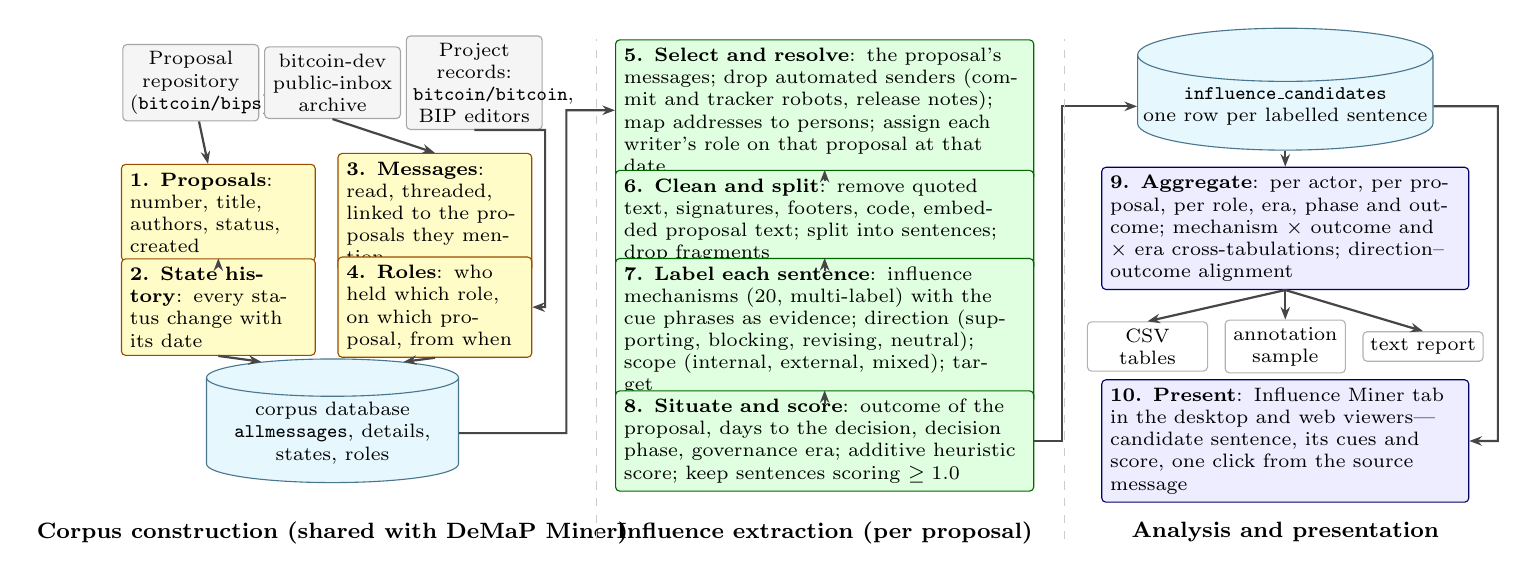
\begin{tikzpicture}[
  font=\scriptsize,
  src/.style={draw=gray!70, rounded corners=1.5pt, fill=gray!8, align=center, inner sep=2.5pt, text width=1.55cm, minimum height=9mm},
  stepA/.style={draw=orange!60!black, rounded corners=1.5pt, fill=yellow!22, align=left, inner sep=3pt, text width=2.25cm},
  stepB/.style={draw=green!40!black, rounded corners=1.5pt, fill=green!12, align=left, inner sep=3pt, text width=5.1cm},
  stepC/.style={draw=blue!40!black, rounded corners=1.5pt, fill=blue!7, align=left, inner sep=3pt, text width=4.45cm},
  db/.style={cylinder, shape border rotate=90, draw=cyan!50!black, fill=cyan!10, aspect=0.18, align=center, inner sep=2pt, minimum width=3.2cm, minimum height=1.05cm},
  outb/.style={draw=gray!60, rounded corners=1.5pt, fill=white, align=center, inner sep=2.5pt, text width=1.35cm},
  arr/.style={-{Stealth[length=1.6mm]}, thick, gray!55!black},
  num/.style={font=\scriptsize\bfseries},
  phase/.style={font=\footnotesize\bfseries, anchor=north},
]
% ================= Phase A: corpus =================
\node[src] (s1) at (0.85,5.2) {Proposal repository \\ (\texttt{bitcoin/bips})};
\node[src] (s2) at (2.65,5.2) {bitcoin-dev public-inbox archive};
\node[src] (s3) at (4.45,5.2) {Project records: \texttt{bitcoin/bitcoin}, BIP editors};
\node[stepA] (a1) at (1.2,3.55) {\textbf{1. Proposals}: number, title, authors, status, created};
\node[stepA] (a2) at (1.2,2.35) {\textbf{2. State history}: every status change with its date};
\node[stepA] (a3) at (3.95,3.55) {\textbf{3. Messages}: read, threaded, linked to the proposals they mention};
\node[stepA] (a4) at (3.95,2.35) {\textbf{4. Roles}: who held which role, on which proposal, from when};
\node[db] (dbA) at (2.65,0.75) {corpus database \\ \texttt{allmessages}, details, \\ states, roles};
\draw[arr] (s1) -- (a1);
\draw[arr] (s2.south) -- (a3.north); \draw[arr] (s3.south) -- (5.35,4.6) -- (5.35,2.35) -- (a4.east);
\draw[arr] (a2.south) -- (dbA.north west); \draw[arr] (a4.south) -- (dbA.north east);
\draw[arr] (a1) -- (a2);
% ================= Phase B: extraction =================
\node[stepB] (b5) at (8.9,4.85) {\textbf{5. Select and resolve}: the proposal's messages; drop automated senders (commit and tracker robots, release notes); map addresses to persons; assign each writer's role on that proposal at that date};
\node[stepB] (b6) at (8.9,3.45) {\textbf{6. Clean and split}: remove quoted text, signatures, footers, code, embedded proposal text; split into sentences; drop fragments};
\node[stepB] (b7) at (8.9,2.05) {\textbf{7. Label each sentence}: influence mechanisms (20, multi-label) with the cue phrases as evidence; direction (supporting, blocking, revising, neutral); scope (internal, external, mixed); target};
\node[stepB] (b8) at (8.9,0.65) {\textbf{8. Situate and score}: outcome of the proposal, days to the decision, decision phase, governance era; additive heuristic score; keep sentences scoring $\geq 1.0$};
\draw[arr] (dbA.east) -- (5.62,0.75) -- (5.62,4.85) -- (b5.west);
\draw[arr] (b5) -- (b6); \draw[arr] (b6) -- (b7); \draw[arr] (b7) -- (b8);
% ================= Phase C: analysis =================
\node[db] (dbC) at (14.75,4.9) {\texttt{influence\_candidates} \\ one row per labelled sentence};
\node[stepC] (c9) at (14.75,3.35) {\textbf{9. Aggregate}: per actor, per proposal, per role, era, phase and outcome; mechanism $\times$ outcome and $\times$ era cross-tabulations; direction--outcome alignment};
\node[outb] (o1) at (13.0,1.85) {CSV tables};
\node[outb] (o2) at (14.75,1.85) {annotation sample};
\node[outb] (o3) at (16.5,1.85) {text report};
\node[stepC] (c10) at (14.75,0.65) {\textbf{10. Present}: Influence Miner tab in the desktop and web viewers---candidate sentence, its cues and score, one click from the source message};
\draw[arr] (b8.east) -- ++(0.35,0) |- (dbC.west);
\draw[arr] (dbC) -- (c9);
\draw[arr] (c9.south) -- (o1.north); \draw[arr] (c9.south) -- (o2.north); \draw[arr] (c9.south) -- (o3.north);
\draw[arr] (dbC.east) -- (17.45,4.9) -- (17.45,0.65) -- (c10.east);
% ================= phase labels =================
\node[phase] at (2.65,-0.25) {Corpus construction (shared with DeMaP Miner)};
\node[phase] at (8.9,-0.25) {Influence extraction (per proposal)};
\node[phase] at (14.75,-0.25) {Analysis and presentation};
\draw[gray!40, dashed] (6.0,-0.6) -- (6.0,5.75);
\draw[gray!40, dashed] (11.95,-0.6) -- (11.95,5.75);
\end{tikzpicture}
\caption{Influence Miner methodology. Steps 1--4 build the DeMaP Miner corpus from the project's repositories, archives and rosters; steps 5--8 turn each proposal's messages into labelled and scored influence candidates; steps 9--10 aggregate and present them. The candidate table is the unit of analysis for all research questions.}
\Description{A three-phase flow diagram. On the left, three sources (proposal repository, mailing-list archives, project records) feed four numbered steps that populate a corpus database. In the middle, four numbered steps select and resolve messages, clean and split them into sentences, label each sentence with mechanisms, direction, scope and target, and situate and score it, producing an influence-candidates table on the right. On the right, an aggregation step produces CSV tables, an annotation sample and a text report, and a presentation step shows the candidates in the desktop and web viewers.}
\label{fig:pipeline}
\end{figure*}

\paragraph{Steps 1--4: corpus construction.} The proposal repository is cloned and each proposal document's preamble parsed for its number, title, authors, current status and creation date (step~1); every commit that changes a status line yields a dated state transition, giving the state history that the study uses to fix the decision date of each proposal (step~2) \cite{sharma2022demap}. The discussion archives are read into a MySQL table with one row per message, with sender, date, subject, thread and body, and each message is linked to the proposals it mentions by number in the subject or body, so that a message about two proposals appears once for each (step~3). The project's own records---the rosters of developers with commit rights, editors, delegates and council members, and the dates on which each was appointed and left---are loaded as role tables, and a post-reading script assigns every message--proposal row the role its writer held on that proposal on that day (step~4). These four steps are the DeMaP Miner corpus and are shared with Rationale Miner and Preference Miner; Section~\ref{sec:corpus} describes how they were carried out for Bitcoin.

\paragraph{Steps 5--8: influence extraction.} For each proposal the tool selects its linked messages, discards messages from automated senders, resolves each writer to a person (a person may write from several addresses) and reads the role from the corpus (step~5, Sections~\ref{sec:filtering} and \ref{sec:roles}). Each message body is then cleaned of quoted text, signatures, list footers, code and embedded proposal text and split into sentences (step~6, Section~\ref{sec:cleaning}). Each sentence is then labelled by four rule-based detectors (step~7, Section~\ref{sec:classification}): the \emph{mechanism} detector assigns any number of the twenty influence mechanisms of Section~\ref{sec:taxonomy} by matching cue phrases with disambiguating context, and records the cues that fired as evidence; the \emph{direction} detector decides whether the sentence supports, blocks or seeks to revise the proposal or is neutral; the \emph{scope} detector decides whether the influence invoked is internal to the project's governance, external to it, or mixed; and the \emph{target} detector names what is being influenced (the proposal, its implementation, governance, compatibility, security, the ecosystem or users). Finally each sentence is situated in the life of its proposal---the proposal's outcome, the number of days between the message and the decision, the decision phase, the governance era---and given an additive heuristic score that rewards mechanisms, decision and justification language, an explicit reference to the proposal, a non-neutral direction, a resolved scope and target, the writer's formal role and proximity to the decision; sentences scoring at least 1.0 are stored as \emph{influence candidates} with all their labels (step~8, Sections~\ref{sec:features} and \ref{sec:scoring}). A sentence with no mechanism is never a candidate; the score orders candidates rather than selects them, and the threshold only removes sentences that carry a mechanism and nothing else.

\paragraph{Steps 9--10: analysis and presentation.} The candidate table is aggregated into per-actor and per-proposal summaries and into the distributions and cross-tabulations that answer the research questions---mechanisms by role, era, phase and outcome, direction against outcome---and exported as CSV files, a stratified annotation sample for human validation, and a plain-text report (step~9, Section~\ref{sec:outputs}). The same table drives the Influence Miner tab of the desktop and web viewers, where an analyst filters candidates by mechanism, direction, role or era and opens the source message of any candidate in its thread (step~10; both viewers read the Bitcoin database unchanged, Section~\ref{sec:adaptation}).

\paragraph{A worked example.} Six weeks before BIP~70 (the payment protocol) was marked Final, its author Gavin Andresen wrote on bitcoin-dev: ``Consensus is the spec should be clarified to match current behavior, so it won't change.'' Step~5 resolves the writer and gives him the role \emph{proposal author} on that date (he had handed over the lead-maintainer role three weeks earlier); step~6 isolates the sentence from the quoted text around it; step~7 labels it \emph{functional} (cue \emph{behavior}), \emph{standards} (cue \emph{spec}) and \emph{coalition} (cue \emph{consensus is}), direction \emph{revising} (cue \emph{clarified}), scope \emph{internal} and target \emph{proposal}; step~8 attaches the outcome \emph{final}, 44 days to the decision and the phase \emph{revision}, and scores it 4.1 (three mechanisms 1.2, decision language +0.6, reference to the spec +0.5, non-neutral direction +0.4, internal scope +0.2, target +0.3, author role +0.7, within ninety days of the decision +0.2). In step~9 it counts once towards each of its three mechanisms and towards the authors' revising signals in the revision phase; in step~10 it is among the top-ranked candidates of BIP~70 in the viewer.

The rest of this section describes each step as built. Influence Miner is implemented in Java as an extension of DeMaP Miner, following the design of Preference Miner, and reads the same MySQL corpus.

\subsection{Data Source and Message Filtering}
\label{sec:filtering}

Messages are read from DeMaP Miner's \texttt{allmessages} table, which links mailing-list messages to PEP numbers by explicit references and subject matching \cite{sharma2022demap}. Column names are discovered at run time so that the same code can be pointed at a BIP database. Two classes of messages are excluded because they carry no human discussion: commit notifications from \texttt{python-checkins} (which embed entire PEP texts and would otherwise account for the majority of extracted sentences) and the bug- and patch-tracker robots (\texttt{report@bugs.python.org}, \texttt{noreply@sourceforge.net}). The exclusion lists are configurable. Messages that mention several PEPs appear once per PEP; duplicates within a PEP are collapsed.

\subsection{Identity and Role Resolution}
\label{sec:roles}

Actor identity is the person, not the address. The corpus provides a clustered display name and a pre-computed role per message; for the rows imported by a newer loader (chiefly 2017--2018, including the whole PEP~572 discussion) we found that the sender-address columns are shifted by one row---they belong to the \emph{next} message---while the clustered name and role agree with the raw ``From:'' header stored with the message body (Section~\ref{sec:threats}). Influence Miner detects these rows, keeps the name and role, and takes the address from the raw header. Roles are then resolved in layers: an optional manual, time-bounded mapping file; the role recorded on the message (BDFL, BDFL delegate, core developer, PEP editor, community member); proposal-specific roles from PEP metadata (proposal author, BDFL delegate); project-wide tables of core developers and PEP editors with their appointment dates; and well-known identities. Proposal-specific roles take precedence over project-wide ones, following the corpus's own convention, except that the BDFL keeps that role. Actors are keyed by the clustered name, which merges one person's several addresses.

\subsection{Text Cleaning and Sentence Splitting}
\label{sec:cleaning}

Each message body is cleaned before splitting: quoted lines, ``On \ldots wrote:'' introductions, forwarded header blocks, message-id and address debris, signature blocks, mailing-list footers, embedded PEP text attachments, code, diffs and tracebacks are removed, and URLs are replaced by a placeholder. Sentences are split on terminal punctuation with protection for abbreviations, version numbers and proposal references; short vote lines such as ``+1'' and ``$-$1'' are kept as sentences. A noise filter drops fragments shorter than three words, sentences longer than 120 words and lines that are mostly non-alphabetic. Cleaning is deliberately conservative: the research depends on real discussion content.

\subsection{Classification}
\label{sec:classification}

Four rule-based detectors label each sentence. The \emph{type} detector matches cue phrases for the twenty mechanisms (thirteen base, seven controversial) on word boundaries, accepts British and American spellings, requires disambiguating context for broad words (``break'' only near compatibility vocabulary, ``risk'' only near security vocabulary, ``team'' only near release or core vocabulary), and records the cue phrases that fired as \emph{evidence}, so that every label can be traced. The \emph{direction} detector is conservative: it classifies a sentence as supporting or blocking only on explicit stance phrases or votes, resolves negations (``I don't object'' is supporting, ``I can't support'' is blocking), treats a sentence with both supporting and blocking cues as ambiguous, demotes hedged sentences and questions, and otherwise assigns revising (revise, defer, clarify, narrow, alternative, compromise \ldots) or neutral. The \emph{scope} detector combines the author's role with actor words in the sentence; role alone never yields ``external''. The \emph{target} detector assigns governance, implementation, security, compatibility, ecosystem, users or proposal.

\subsection{Outcome, Temporal Features and Scoring}
\label{sec:features}

The proposal outcome is resolved from the corpus's table of accepted and rejected PEPs and, for the remaining PEPs, from the PEP state history mined from the PEP repository log, normalised to accepted, rejected, withdrawn, deferred, final, active, superseded, draft, provisional or unknown, with the decision timestamp. From the decision date and the PEP creation date the tool computes the number of days between the message and the decision and a coarse decision phase (pre-draft, early discussion, active debate, revision, decision window, post-decision). A configurable governance split date (default 12~July~2018, when Guido van Rossum stepped down) assigns each message to the BDFL or post-BDFL era. Direction is compared with outcome to obtain an \emph{alignment} flag: supporting signals align with accepted, final or active proposals; blocking with rejected, withdrawn or deferred ones; revising with deferred, superseded, draft or provisional ones.

A transparent additive score combines the number of mechanisms detected, deontic and decision language, justification language, explicit reference to the proposal, a non-neutral direction, a resolved scope and target, the author's formal role, and proximity to the decision (only when the decision date is known and the message precedes it), with penalties for hedging and very short sentences. Sentences scoring at least 1.0 are stored as candidates with all labels, evidence cues, role, outcome and temporal features.

\subsection{Aggregation and Outputs}
\label{sec:outputs}

A batch runner processes one proposal, a range or the whole corpus, continues after errors and logs per-proposal statistics. An aggregator populates per-actor and per-proposal summary tables and computes multi-label type distributions, direction, scope, role, phase and era distributions, type-by-outcome and type-by-era cross-tabulations and alignment counts. An exporter writes these as CSV files; a sampler exports a stratified annotation sheet (top-scored, random, per-type and per-outcome strata) with empty human-label columns; and a report generator writes a plain-text summary. All code, SQL and configuration are in the DeMaP Miner repository.

\subsection{Scoring in Detail}
\label{sec:scoring}

The heuristic score is additive and every component is inspectable. A candidate starts at 0.8 for carrying at least one mechanism (+0.2 for a second, +0.2 for a third); +0.6 for deontic or decision language (\emph{should, must, need to, recommend, object, reject, accept, agree, insist, strongly, clearly}); +0.4 for justification language (\emph{because, therefore, for example, evidence, in practice, in my experience, shows that}); +0.5 for an explicit reference to the proposal (\emph{PEP~572, this change, this syntax, the spec}); +0.4 for a non-neutral direction; +0.2 for an internal or external scope and +0.4 for a mixed one; +0.3 for a recognised target; a role weight of 1.0 for the BDFL or Steering Council, 0.9 for a delegate, 0.8 for a core developer or release manager, 0.7 for a proposal author or PEP editor, 0.2 for a community member; +0.8, +0.5 or +0.2 when the message precedes a known decision by at most 7, 30 or 90 days; $-$0.2 for hedging (\emph{maybe, perhaps, not sure, I wonder}) and $-$0.3 for sentences shorter than six words unless they are votes. Unknown decision dates and post-decision messages add nothing, so proposals without a resolved decision are not boosted. The threshold of 1.0 keeps every sentence with a mechanism and at least one further signal; the annotation study will tell whether it should be raised.

\subsection{Adapting the Tool to Bitcoin}
\label{sec:adaptation}

The pipeline above was written for the Python corpus and ran on the Bitcoin corpus after four changes, none of which touches the classifiers. First, the table and column names that identify a proposal are derived from the proposal identifier (\texttt{accrejbips}, \texttt{bipdetails}, \texttt{bipeditors}, column \texttt{BIP}), so the same code reads either database. Second, the outcome resolver understands the BIP status vocabulary, including the 2025 revision (Section~\ref{sec:corpus}). Third, the role mapper knows the \emph{lead maintainer} role, which takes the BDFL's weight in the score, and reads Bitcoin's roster tables; the message-level role labels are computed by a post-reading script from those rosters exactly as for Python. Fourth, the cue lists were extended with Bitcoin's own governance vocabulary---its decision-makers (\emph{lead maintainer, core maintainers, BIP editors} and the handles of the best-known maintainers) for \emph{authority}, the companies and funders active in the project for \emph{corporate interest}, chain splits and client switching for \emph{exit threat}, list moderation and censorship complaints for \emph{procedural control}, and the flame vocabulary of the block-size war (\emph{shill, scam, sockpuppet, brigading, bad faith}) for \emph{incivility} (Appendix~\ref{app:rules}). Release announcements, whose release notes enumerate dozens of BIPs and are not discussion, are skipped by a subject filter, as commit notifications were skipped for Python; without it the lead maintainer's release notes alone would have contributed more than 5,000 candidate sentences. Both user interfaces read the Bitcoin database unchanged.

\section{Study Design}
\label{sec:design}

\subsection{Building the Bitcoin Corpus}
\label{sec:corpus}

The corpus was rebuilt from public sources so that it covers the whole life of the list and can be regenerated. Table~\ref{tab:sources} summarises it.

\begin{table}[t]
\caption{Sources of the Bitcoin corpus (June 2011 to September 2026).}
\label{tab:sources}
\footnotesize
\setlength{\tabcolsep}{3.5pt}
\begin{tabular}{p{0.46\columnwidth}p{0.48\columnwidth}}
\toprule
Source & Content \\
\midrule
bitcoin-dev public-inbox mirror (gnusha.org) & 24,663 messages, 2011-06-11 to 2026-09-11, spanning the SourceForge, Linux Foundation and Google Groups eras; 24,391 read, 6,886 linked to a BIP number (11,477 message--BIP rows, 205 BIPs) \\
\texttt{bitcoin/bips} repository & 211 BIP documents (preamble: number, title, authors, status, type, layer, created) and 505 status changes for 197 BIPs from the git history \\
\texttt{bitcoin/bitcoin} repository & 50,557 commits: merge committers (maintainers, with active dates) and contributors with at least ten commits (from first commit) \\
BIP 1/2/3 and repository history & BIP editors and their terms; lead maintainers and their terms \\
\bottomrule
\end{tabular}
\end{table}

\paragraph{Mailing list.} bitcoin-dev has had three homes: SourceForge (as bitcoin-development, 2011--2015), the Linux Foundation (2015--February 2024) and Google Groups (since February 2024). The public-inbox archive maintained by Bryan Bishop at gnusha.org \cite{gnusha} holds all three as one git repository with one RFC-822 message per blob. It was mirrored with \texttt{git clone --mirror}, every message was exported into a monthly mbox by its \texttt{Date:} header, and the mboxes were converted into the pipermail monthly text format that DeMaP Miner's reader was written for, using the converter built for Python's Mailman~3 archives. One Bitcoin-specific fix was needed: Google Groups rewrites the \texttt{From:} header of every post to the group's own address for DMARC, keeping the real sender in \texttt{X-Original-From}; the converter now prefers that header, without which the 687 posts of the Google Groups era would have been credited to one sender. The reader then linked each message to the BIP numbers it mentions (subject and body, ``BIP 341'', ``BIP-341'', ``bip341''), storing a message once per BIP as it does for PEPs; messages that discuss a proposal before it has a number, or by name only (``Taproot'', ``CTV''), are not linked, which is the main coverage limit of this study and is discussed in Section~\ref{sec:threats}.

\paragraph{Proposal metadata and state history.} The \texttt{bitcoin/bips} repository was cloned and each document's preamble parsed. Two preamble conventions coexist: BIP 2's (\emph{Author}, \emph{Created}, statuses Draft, Proposed, Final, Active, Deferred, Rejected, Withdrawn, Replaced and Obsolete) and BIP 3's, introduced in 2025 (\emph{Authors}, \emph{Assigned}, statuses Draft, Deployed, Complete and Closed). Every commit that changes a \texttt{Status:} line yields a (BIP, from, to, timestamp) record, giving 505 status changes for 197 BIPs. On 12 April 2025 a single commit relabelled every BIP into the new vocabulary (Final $\to$ Deployed or Complete, Rejected/Withdrawn/Obsolete/Replaced $\to$ Closed); the final decision used for RQ4 is therefore the last status \emph{before} that commit where one exists, and the current status otherwise, so that ``Closed'' does not erase the distinction between rejected and withdrawn proposals. The tool's outcome resolver was extended to read the BIP vocabulary (Proposed as a pre-decision state; Deployed and Complete as positive; Closed and Obsolete as negative).

\paragraph{Roles.} Bitcoin has no BDFL, no delegates and no council, so the role vocabulary was rebuilt from the project's own records. The \emph{lead maintainer} (Gavin Andresen to 7 April 2014, Wladimir van der Laan to 31 January 2022) is the closest analogue of Python's BDFL. \emph{Maintainers} are the authors of merge commits in \texttt{bitcoin/bitcoin} (at least twenty merges; the role is time-bounded by their first and last merge), \emph{core developers} are contributors with at least ten non-merge commits from the date of their first commit, \emph{BIP editors} are taken from the history of BIP 1, BIP 2 and the repository's README with their terms (Amir Taaki 2011--2013, Gregory Maxwell 2013--2016, Luke Dashjr 2016--2026, Kalle Alm 2021--2024, and Bryan Bishop, Jon Atack, Mark Erhardt, Olaoluwa Osuntokun and Ruben Somsen from April 2024), and \emph{proposal authors} come from the BIP preambles and hold that role on their own BIP only. Everyone else is a \emph{community member}. Roles are proposal- and date-specific: the same person is an author on their BIP, a maintainer while they merge, and a community member before their first commit. Names were clustered by address and a short alias list (handles such as \emph{sipa}, \emph{gmaxwell}, \emph{luke-jr}, \emph{roasbeef}, \emph{fanquake}, \emph{glozow}, \emph{kanzure}, \emph{murch} map to the person). Per message--BIP row the corpus holds 6,762 community-member, 2,514 core-developer, 1,095 author, 530 editor, 353 maintainer and 223 lead-maintainer rows.

\paragraph{Cross-check against the 2021 database.} The group's earlier Bitcoin database (built in 2021 from the Linux Foundation archives of bitcoin-dev, bitcoin-core-dev and bitcoin-discuss) survives as its sentence and paragraph tables---284,303 sentences from 18,600 messages on 146 BIPs, split into a 50-column feature layout written for reason extraction and topic modelling---and was attached to the same server for comparison. Up to the date of that database (13 May 2021) the rebuilt corpus holds 18,830 bitcoin-dev messages linked to 146 BIPs, against the 18,288 bitcoin-dev messages and 144 BIPs of the 2021 tables; per BIP the counts agree closely (BIP~9: 348 vs.\ 353 messages; BIP~141: 287 vs.\ 283; BIP~341: 37 vs.\ 32). The automated linking therefore reproduces the hand-checked coverage of the earlier study. The two lists the earlier database also read, bitcoin-core-dev and bitcoin-discuss (7\% of its sentences), are not in the rebuilt corpus.

\paragraph{Governance eras.} For RQ3 the split date is 1 February 2022, the end of the lead-maintainer role; the analysis also reports four finer periods---the Andresen years (June 2011 to April 2014), the block-size war (April 2014 to the activation of Segregated Witness on 24 August 2017), the van der Laan years after the war (to January 2022) and the post-lead era (from February 2022)---because the war is the period in which the community's governance was contested most openly.

\subsection{Analysis}

The analysis mirrors the Python study. RQ1 uses the multi-label mechanism distribution, its profile across decision phases and the timing of signals relative to the decision; RQ2 the role distribution and actor-level aggregates; RQ3 the era comparison; RQ4 the mechanism mix by outcome and direction--outcome alignment against the base rate; RQ5 the overlap with preference signals; RQ6 the seven controversial mechanisms, their concentration by role, era, proposal and phase, and the year-by-year landmark acts nominated by the tool. Section~\ref{sec:compare} then sets the Bitcoin profile against the Python profile obtained with the same detector. All statistics are descriptive.


\begin{figure*}[t]
\centering
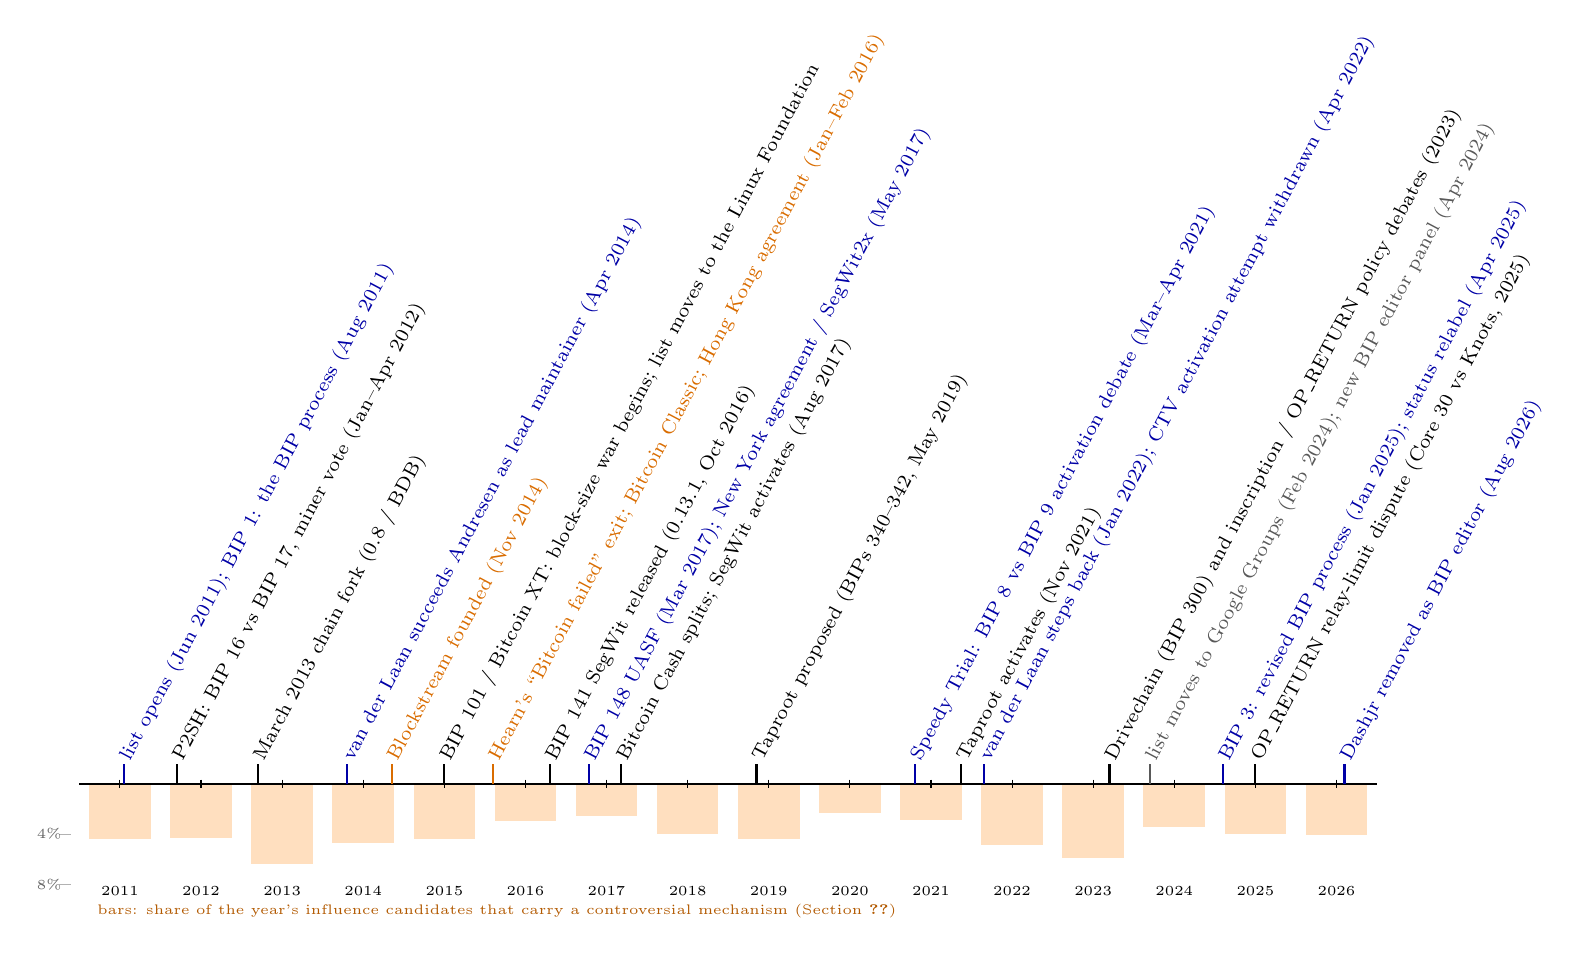
\begin{tikzpicture}[x=1.03cm, y=1cm, font=\scriptsize]
  % ---- yearly share of influence candidates carrying a controversial mechanism (filled by the assembly script) ----
  \foreach \yr/\p in {2011/4.4, 2012/4.3, 2013/6.4, 2014/4.7, 2015/4.4, 2016/3.0, 2017/2.6, 2018/4.0, 2019/4.4, 2020/2.3, 2021/2.9, 2022/4.9, 2023/5.9, 2024/3.4, 2025/4.0, 2026/4.1} {
    \pgfmathsetmacro{\xl}{\yr-2011+0.12}
    \pgfmathsetmacro{\xr}{\yr-2011+0.88}
    \pgfmathsetmacro{\h}{-\p*0.16}
    \fill[orange!25] (\xl,0) rectangle (\xr,\h);
  }
  \draw[gray!60] (-0.25,-0.64) -- (-0.1,-0.64) node[left, text=gray!80!black, font=\tiny] {4\%};
  \draw[gray!60] (-0.25,-1.28) -- (-0.1,-1.28) node[left, text=gray!80!black, font=\tiny] {8\%};
  \node[anchor=west, text=orange!70!black, font=\tiny] at (0.1,-1.62) {bars: share of the year's influence candidates that carry a controversial mechanism (Section~\ref{sec:rq6})};
  % ---- axis and years ----
  \draw[thick] (0,0) -- (16,0);
  \foreach \yr in {2011,2012,...,2026} {
    \draw (\yr-2011+0.5,0.05) -- (\yr-2011+0.5,-0.05);
    \node[font=\tiny] at (\yr-2011+0.5,-1.36) {\yr};
  }
  \tikzset{gov/.style={blue!65!black}, lang/.style={black}, venue/.style={gray!70!black}, corp/.style={orange!85!black}}
  \foreach \x/\c/\t in {
    2011.55/gov/{list opens (Jun 2011); BIP 1: the BIP process (Aug 2011)},
    2012.2/lang/{P2SH: BIP 16 vs BIP 17, miner vote (Jan--Apr 2012)},
    2013.2/lang/{March 2013 chain fork (0.8 / BDB)},
    2014.3/gov/{van der Laan succeeds Andresen as lead maintainer (Apr 2014)},
    2014.85/corp/{Blockstream founded (Nov 2014)},
    2015.5/lang/{BIP 101 / Bitcoin XT: block-size war begins; list moves to the Linux Foundation},
    2016.1/corp/{Hearn's ``Bitcoin failed'' exit; Bitcoin Classic; Hong Kong agreement (Jan--Feb 2016)},
    2016.8/lang/{BIP 141 SegWit released (0.13.1, Oct 2016)},
    2017.28/gov/{BIP 148 UASF (Mar 2017); New York agreement / SegWit2x (May 2017)},
    2017.68/lang/{Bitcoin Cash splits; SegWit activates (Aug 2017)},
    2019.35/lang/{Taproot proposed (BIPs 340--342, May 2019)},
    2021.3/gov/{Speedy Trial: BIP 8 vs BIP 9 activation debate (Mar--Apr 2021)},
    2021.87/lang/{Taproot activates (Nov 2021)},
    2022.15/gov/{van der Laan steps back (Jan 2022); CTV activation attempt withdrawn (Apr 2022)},
    2023.7/lang/{Drivechain (BIP 300) and inscription / OP\_RETURN policy debates (2023)},
    2024.2/venue/{list moves to Google Groups (Feb 2024); new BIP editor panel (Apr 2024)},
    2025.1/gov/{BIP 3: revised BIP process (Jan 2025); status relabel (Apr 2025)},
    2025.5/lang/{OP\_RETURN relay-limit dispute (Core 30 vs Knots, 2025)},
    2026.6/gov/{Dashjr removed as BIP editor (Aug 2026)}} {
    \draw[\c, thick] (\x-2011,0) -- (\x-2011,0.25);
    \node[\c, rotate=62, anchor=west, inner sep=1pt] at (\x-2011,0.27) {\t};
  }
\end{tikzpicture}
\caption{Landmark influences on the Bitcoin project from the start of the corpus (June 2011) to September 2026, above a corpus-derived measure of contestation: the share of each year's influence candidates that carry one of the seven controversial mechanisms (Section~\ref{sec:rq6}). Blue: governance and process; black: protocol decisions; orange: employer, funding and corporate stakes; grey: venues. Dates from the BIP repository, the reference implementation's history and the list itself.}
\label{fig:timeline}
\Description{A horizontal timeline from 2011 to 2026 with colour-coded events rising from the axis at an angle and a bar chart below the axis showing the yearly percentage of controversial influence candidates.}
\end{figure*}
\section{Results}
\label{sec:results}

Table~\ref{tab:corpus} summarises the run. Of the 11,477 message--BIP rows, none came from automated senders; 331 rows (229 messages) were release announcements and were skipped. Cleaning and splitting the rest produced about 205,000 sentences, of which 62,791 (about 31\%) carried at least one mechanism and scored above the threshold: on average 1.38 mechanisms per candidate, from 636 participants on 199 BIPs. Outcomes were resolved for 157 BIPs: 89 final, 22 rejected, 15 withdrawn, 25 draft, 5 superseded, 4 deferred and 3 active; 36 BIPs (2,404 candidates) have no recorded decision.

\begin{table}[t]
\caption{Corpus and extraction summary (Bitcoin).}
\label{tab:corpus}
\small
\begin{tabular}{lr}
\toprule
bitcoin-dev messages read & 24,391 \\
\quad linked to a BIP number & 6,886 (11,477 message--BIP rows) \\
\quad release announcements skipped & 229 messages (331 rows) \\
BIPs with linked messages & 205 \\
Influence candidate sentences stored & 62,791 \\
BIPs with at least one candidate & 199 \\
Distinct participants (actors) & 636 \\
Mechanisms per candidate & 1.38 \\
Period covered & 2011-06 to 2026-09 \\
\bottomrule
\end{tabular}
\end{table}

\subsection{RQ1: Influence Mechanisms}

Table~\ref{tab:rq1} shows how often each base mechanism occurs. Bitcoin's profile is not Python's. \emph{Ecosystem} arguments lead by a wide margin (33.7\% of candidates): what wallets, nodes, miners, exchanges and other implementations will do or suffer is the community's first consideration. \emph{Operational} arguments (22.0\%: implementation, deployment, activation, releases) come second, and then two mechanisms that were marginal in Python: \emph{security} (17.5\%---attacks, chain splits, fund loss, denial of service, malleability) and \emph{economic} (14.8\%---fees, miner incentives, cost, the fee market). \emph{Compatibility} follows (12.1\%: soft and hard forks, non-upgraded nodes, replay protection), and only then \emph{functional} arguments about whether the design solves the problem (7.6\%), which were Python's second mechanism at 25.8\%. \emph{Authority} is invoked in 2.5\% of candidates, a third of Python's 7.6\%, and \emph{coalition} in 2.1\%. Two caveats apply as in Python: the multi-label counts sum to more than 100\%, and \emph{ecosystem} in Bitcoin is inflated by the fact that nodes, wallets and miners are components of the protocol as well as constituencies---a sentence that describes what a node does fires the same cue as one that argues from what node operators will accept. The rank order is nonetheless robust to that inflation: the four Bitcoin-specific mechanisms the taxonomy singled out (ecosystem, security, economic, compatibility) occupy four of the top five places.

\begin{table}[t]
\caption{RQ1: base influence mechanisms in 62,791 candidate sentences (multi-label), with the Python share on the extended corpus for comparison.}
\label{tab:rq1}
\small
\begin{tabular}{lrrr}
\toprule
Mechanism & Candidates & \% Bitcoin & \% Python \\
\midrule
Ecosystem & 21,151 & 33.7 & 18.4 \\
Operational & 13,812 & 22.0 & 27.0 \\
Security & 10,976 & 17.5 & 2.6 \\
Economic & 9,324 & 14.8 & 2.3 \\
Compatibility & 7,568 & 12.1 & 13.6 \\
Functional & 4,755 & 7.6 & 25.8 \\
Standards & 4,095 & 6.5 & 8.8 \\
Organizational & 2,796 & 4.5 & 3.2 \\
Strategic & 2,667 & 4.2 & 5.0 \\
Tactical & 2,065 & 3.3 & 4.9 \\
User demand & 1,976 & 3.1 & 3.6 \\
Authority & 1,596 & 2.5 & 7.6 \\
Coalition & 1,317 & 2.1 & 2.0 \\
\bottomrule
\end{tabular}
\end{table}

Table~\ref{tab:samples} shows two sentences per mechanism as the tool extracted and labelled them. They illustrate what the labels mean in Bitcoin: an ecosystem argument is a claim about miners, wallets or a chain split (``If miners interpret the situation as being forced to run non-reference software in order to prevent a chain split \ldots that could be a one-way street''); a security argument is about fund loss and attacks (``Wallets can't share keys unless their functionality is identical, half-interoperability can lead to funds loss''); an economic argument is about fees and incentives (``it's miner-incentive compatible''); an authority argument names the BIP editors or the maintainers rather than a person with the power to decide.

\begin{table*}[t]
\caption{Sample sentences per base mechanism as extracted and labelled by Influence Miner (Bitcoin corpus). Multi-label; the mechanism shown is one of those assigned.}
\label{tab:samples}
\small
\begin{tabular}{p{0.10\textwidth}p{0.155\textwidth}p{0.69\textwidth}}
\toprule
Mechanism & BIP, author (role) & Sentence \\
\midrule
Strategic & 101, Garzik (core dev.) & Many miners, for example, openly state they prefer long term system growth over maximizing tiny amounts of current day income. \\
Strategic & 341, symphonicbtc (community) & It is important to consider that miners are not always incentivized by what brings them the most profit in the moment, but also their long-term prospects. \\
Operational & 32, Hearn (core dev.) & I definitely want to implement HD wallets in bitcoinj to allow this and if that means not using the same tree structure as in the BIP then so be it. \\
Operational & 148, Alm (core dev.) & One thing about BIP148 activation that may be affected by this is the fact that segwit signalling non-BIP148 miners + BIP148 miners may hold majority hash power and prevent a chain split. \\
Functional & 44, Maxwell (core dev.) & Wallets can't share keys unless their functionality is identical, half-interoperability can lead to funds loss. \\
Functional & 34, Wuille (maintainer) & I believe we should get rid of checkpoints because they seem to be misunderstood as a security feature rather than as an optimization. \\
Tactical & 91, Aronesty (community) & The BIP should be modified to provide evidence and justification for the timeline that is consistent with the level of risk the network would bear if it were enacted. \\
Tactical & 148, Eliosoff (community) & Unless the HF code is ready and agreed on soon (say by Jul 1), my vote is to keep the main chain backwards-compatible, especially if evidence of miner support for BIP148 doesn't materialize soon. \\
Authority & 2, Corallo (core dev.) & While there are plenty of competent technical folks who would make fine BIP editors, I'd suggest Kanzure and Murch as clear candidates over others. \\
Authority & 8, Tim\'on (core dev.) & I think the option of ``permanent failure because miners veto'' should actually be abandoned. \\
Compatibility & 9, Lau (core dev.) & To avoid risks of fund loss, users MUST NOT create P2WSH scripts that are incompatible with this BIP. \\
Compatibility & 148, Dashjr (BIP editor) & Replay protection is equally a concern for the main (BIP148) chain and any legacy chains malicious miners might choose to split off. \\
Security & 91, Hilliard (author) & Since this BIP only activates with a clear miner majority it should not increase the risk of an extended chain split. \\
Security & 65, Tim\'on (core dev.) & Can you give an example of an attack in which a non-upgraded full node wallet is defrauded with BIP65 but could not with the hardfork alternative? \\
Standards & 68, Todd (core dev.) & If it had done that, that text would be part of a ``Standard BIP'' rather than ``Informational BIP'', thus I'll argue that BIP9 should also be a ``Standard BIP''. \\
Standards & 39, Provoost (core dev.) & Wallets need to be able to distinguish between the old and new standard, so un-upgraded BIP 39 wallets should consider all new mnemonics invalid. \\
Ecosystem & 148, Friedenbach (core dev.) & If miners interpret the situation as being forced to run non-reference software in order to prevent a chain split because a lack of support from Bitcoin Core, that could be a one-way street. \\
Ecosystem & 70, Andresen (lead maint.) & If the spec said that wallets must not broadcast until they receive a PaymentACK, then you'd have to violate the spec to do CoinJoin. \\
Economic & 125, Ruane (core dev.) & An advantage of this mempool-accept policy change is that it's miner-incentive compatible (miners would prefer to mine a transaction with a higher feerate). \\
Economic & 109, Towns (core dev.) & Likewise we don't want to have miners or pool operators have to take responsibility for managing the whole economy, rather than just keeping their systems running. \\
Organizational & 101, Hearn (core dev.) & I agree with Gavin---whilst it's great that a Blockstream employee has finally made a realistic proposal (i.e.\ not ``let's all use Lightning'')---this BIP is virtually the same as keeping the 1mb cap. \\
Organizational & 62, Maxwell (BIP editor) & If you are running third-party or self-compiled Bitcoin Core or an alternative implementation using OpenSSL you must not update OpenSSL or must run a Bitcoin software containing a workaround. \\
Coalition & 70, Andresen (author) & Consensus is the spec should be clarified to match current behavior, so it won't change. \\
Coalition & 38, Dashjr (BIP editor) & For example, many people seem to think BIP 38 is a good idea simply because it is a Final BIP, whereas in general we would want to discourage using it since it cannot really be used safely. \\
User demand & 70, Hearn (author) & Whilst having an extension cannot really hurt, obviously, BIP70 will not be amended to reduce the certificate types it allows in favour of a system that has a very low chance of mainstream adoption. \\
User demand & 62, Hearn (core dev.) & Although I agree not having to support all of DER is nice, in practice I think all implementations do and libraries to parse DER are widespread. \\
\bottomrule
\end{tabular}
\end{table*}

\paragraph{Direction and scope.} Direction is neutral for 88.5\% of candidates, revising for 8.7\%, supporting for 1.5\% and blocking for 1.4\%---almost exactly Python's distribution (87.7 / 8.8 / 2.0 / 1.5). Scope differs: 17.6\% of Bitcoin's candidates are \emph{external} and 10.0\% \emph{mixed}, against 3.0\% and 4.7\% in Python, because Bitcoin's arguments name users, wallets, exchanges, miners and companies far more often; 32.8\% are internal and 39.7\% unresolved.

\paragraph{When influence is exercised.} The temporal profile is where the two projects differ most, and the difference is instructive. In Python, signalling peaked sharply in the four weeks around the recorded decision. In Bitcoin only 102 candidates (0.2\%) fall in the two weeks before the recorded decision and 3.1\% in the first month after a BIP's creation; 56.7\% are ``active debate'' and 36.5\% post-decision. The reason is that a BIP's recorded status change is not the moment of its decision. Consensus BIPs become \emph{Final} when they are deployed and activated, often years after the debate (BIP~141 was discussed in 2015--2017 and marked Final in August 2017, BIP~341 in February 2023), and many early BIPs received their terminal status in bulk clean-ups of the repository (5 on 21 October 2013, 13 on 1 February 2016, 15 on 10 July 2024, 24 on 12 April 2025). The decision in Bitcoin is made in the ecosystem---by what is merged, released, signalled and run---and the repository records it afterwards; the tool's decision-window phase, which worked for Python because the BDFL's pronouncement and the PEP's status change coincide, has no counterpart here. Mechanism shares are accordingly flat across phases (ecosystem 34.5\% in active debate, 32.7\% after the decision; security 16.4\% and 19.8\%; economic 16.1\% and 12.9\%), with authority and standards higher only in the small early-discussion and pre-draft phases (6.3\% and 8.3\%).

\subsection{RQ2: Who Exercises Influence}

Table~\ref{tab:roles} gives the candidates by role. Community members---participants who are neither authors of the BIP under discussion, nor Bitcoin Core contributors, maintainers or editors---write 57.6\% of Bitcoin's influence candidates, against 37\% in Python; core developers 27.1\%, proposal authors 9.8\%, BIP editors 2.4\%, maintainers 2.0\% and the lead maintainer 1.0\%. The last figure is the starkest contrast with Python, where the BDFL alone wrote 8--11\% of candidates: Gavin Andresen and Wladimir van der Laan together account for 655 candidate sentences on 45 BIPs, and after 2015 the lead maintainer disappears from the list altogether (0.0\% of candidates in every year from 2016), his contributions being the release announcements that the tool sets aside. Bitcoin's decisions were not argued by its formal leaders. The roles differ in what they argue about: editors and maintainers invoke authority most (5.5\% and 3.7\%) and security least among the developer roles; community members and core developers carry the highest security shares (17.9\% and 18.1\%); economic arguments are made by everyone except the editors (7.9\%). Average scores rise with role weight as designed (community 1.67, core developer 2.42, editor 2.64).

\begin{table}[t]
\caption{RQ2: candidates by author role, with each role's share of authority, security and economic mechanisms (\%).}
\label{tab:roles}
\small
\setlength{\tabcolsep}{4pt}
\begin{tabular}{lrrrrrr}
\toprule
Role & Cand. & \% & People & Auth. & Sec. & Econ. \\
\midrule
Community member & 36,139 & 57.6 & 597 & 2.3 & 17.9 & 13.7 \\
Core developer & 17,045 & 27.1 & 48 & 2.8 & 18.1 & 17.4 \\
Proposal author & 6,179 & 9.8 & 67 & 1.9 & 16.3 & 16.6 \\
BIP editor & 1,530 & 2.4 & 7 & 5.5 & 12.4 & 7.9 \\
Maintainer & 1,245 & 2.0 & 9 & 3.7 & 13.5 & 13.3 \\
Lead maintainer & 655 & 1.0 & 2 & 4.4 & 7.8 & 15.3 \\
\bottomrule
\end{tabular}
\end{table}

The most active individuals are core developers and long-standing community members rather than office-holders: Antoine Riard (about 3,700 candidates on 64 BIPs), Anthony Towns (1,900 on 58), Eric Voskuil (1,800 on 49), the pseudonymous \emph{conduition} (1,700 on 19), Peter Todd (1,400 on 51), Johnson Lau (3,000 across his roles as core developer, author and community member), Jorge Tim\'on (1,100 on 35), Matt Corallo (950 on 59) and Mike Hearn (800 on 17). Direction does not vary by role (supporting 0.8--2.6\%, blocking 0.7--1.6\%, revising 6.6--9.1\%); maintainers are the most supportive (2.6\%) and least blocking (0.7\%) role, the lead maintainer the least supportive (0.8\%).

\subsection{RQ3: Governance Periods}

Table~\ref{tab:eras} compares the four periods. Two things stay constant: the ordering of the top mechanisms (ecosystem, operational, then security or economic) and the near-absence of authority (4.5\% in the Andresen years, 1.5--3.0\% afterwards). Three things change. First, the block-size war has the highest \emph{compatibility} share of any period (18.3\%, against 7--10\% before and after): the war was argued as a question of what a hard fork would break and whom it would leave behind. Second, \emph{security} rises steadily from 12.9\% to 22.4\% and \emph{economic} from 10.1\% to 17.9\% across the four periods, so that in the post-lead era the two together outweigh operational arguments; the covenant, relay-policy and quantum-resistance debates of 2022--2026 are argued in terms of attacks and incentives. Third, the share of the lead maintainer, maintainers and editors in the conversation shrinks from 17.8\% of candidates in the Andresen years to 3.4\% in the post-lead era while core developers grow from 20.7\% to 33.6\%; in 2024 core developers wrote 56\% of all candidates. Whether the war's end changed the register can be read from the drop in controversial mechanisms from 5.8\% (Andresen years) to 3.4\% (war) and 3.2\% (post-war), and their rise again to 4.6\% in the post-lead era (Section~\ref{sec:rq6}).

\begin{table}[t]
\caption{RQ3: mechanism shares (\%) and role shares (\%) by governance period.}
\label{tab:eras}
\footnotesize
\setlength{\tabcolsep}{3pt}
\begin{tabular}{lrrrr}
\toprule
 & Andresen & Block-size war & van der Laan & Post-lead \\
 & 2011--14 & 2014--17 & 2017--22 & 2022--26 \\
\midrule
Candidates & 3,472 & 21,713 & 14,900 & 22,706 \\
BIPs & 33 & 101 & 106 & 131 \\
Participants & 102 & 270 & 225 & 243 \\
\midrule
Ecosystem & 33.4 & 37.8 & 34.9 & 28.8 \\
Operational & 18.6 & 22.8 & 25.3 & 19.5 \\
Security & 12.9 & 13.7 & 16.3 & 22.4 \\
Economic & 10.1 & 12.3 & 14.8 & 17.9 \\
Compatibility & 7.1 & 18.3 & 9.5 & 8.5 \\
Functional & 10.5 & 6.1 & 8.7 & 7.7 \\
Standards & 11.3 & 5.2 & 7.6 & 6.3 \\
Authority & 4.5 & 3.0 & 1.5 & 2.5 \\
Strategic & 4.5 & 3.7 & 4.3 & 4.7 \\
Coalition & 1.6 & 2.3 & 2.2 & 1.9 \\
\midrule
Lead maint.\ + maint.\ + editors & 17.8 & 6.8 & 3.8 & 3.4 \\
Core developers & 20.7 & 22.3 & 25.7 & 33.6 \\
Community members & 50.3 & 59.3 & 61.6 & 54.5 \\
\midrule
Any controversial & 5.8 & 3.4 & 3.2 & 4.6 \\
\bottomrule
\end{tabular}
\end{table}

\subsection{RQ4: Alignment with Outcomes}

Because 75\% of candidates sit on BIPs that became final, outcome comparisons rest on smaller groups (Table~\ref{tab:outcomes}). Rejected BIPs attract proportionally more \emph{compatibility} (20.1\% vs.\ 12.1\% on final BIPs), \emph{economic} (18.4\% vs.\ 14.4\%) and \emph{authority} (5.6\% vs.\ 1.8\%) signals and fewer \emph{security} (9.1\% vs.\ 17.7\%) and \emph{operational} (17.2\% vs.\ 22.7\%) ones: proposals fail in Bitcoin when they are argued to break things, to misalign incentives, or to need someone's permission, and succeed when the discussion has moved to attacks and implementation. Draft BIPs carry the most security (26.8\%) and economic (21.0\%) argument---the covenant and quantum proposals still under discussion---and superseded BIPs the most authority and strategic argument (8.6\% each). Direction--outcome alignment is 74.9\% for supporting sentences, 12.1\% for blocking and 9.7\% for revising, against a base rate of 76\% of decided candidates on positive outcomes; as in Python, counting explicit stances predicts nothing, and in Bitcoin the blocking figure is lower still because so few discussed BIPs are formally rejected---objections that succeed leave a BIP a draft forever rather than ``Rejected''.

\begin{table}[t]
\caption{RQ4: mechanism share (\%) by proposal outcome.}
\label{tab:outcomes}
\small
\setlength{\tabcolsep}{4pt}
\begin{tabular}{lrrrr}
\toprule
Mechanism & Final (89) & Rejected (22) & Withdrawn (15) & Draft (25) \\
\midrule
Ecosystem & 35.1 & 35.0 & 32.8 & 26.7 \\
Operational & 22.7 & 17.2 & 22.6 & 18.7 \\
Security & 17.7 & 9.1 & 12.9 & 26.8 \\
Economic & 14.4 & 18.4 & 14.9 & 21.0 \\
Compatibility & 12.1 & 20.1 & 14.2 & 7.5 \\
Functional & 7.4 & 5.8 & 8.0 & 8.8 \\
Standards & 6.9 & 3.2 & 4.0 & 5.3 \\
Authority & 1.8 & 5.6 & 4.5 & 2.1 \\
Organizational & 4.1 & 5.0 & 6.3 & 4.9 \\
Strategic & 4.0 & 4.8 & 3.7 & 4.3 \\
\bottomrule
\end{tabular}
\end{table}

\subsection{RQ5: Complementarity with Preference Miner}

Preference Miner has not yet been run on the rebuilt Bitcoin corpus, so the overlap measured for Python (1.6\% of influence sentences coincide with preference sentences) cannot be reported for Bitcoin. The two tools read the same tables and the Bitcoin database carries the same schema, so the comparison requires only a Preference Miner run; it is left for the next iteration.

\subsection{RQ6: Controversial Influence}
\label{sec:rq6}

\paragraph{How much and which.} 2,458 candidates (3.9\%) carry at least one of the seven controversial mechanisms, slightly fewer than Python's 4.7\% (Table~\ref{tab:rq6}). The ordering is Python's with one change: incivility leads (1.43\%), then procedural control (0.78\%) and backchannel references (0.73\%), but corporate interest (0.49\%) comes next and ahead of unilateral decisions (0.22\%), which in Python were twice as frequent as corporate stakes. Gatekeeping (0.17\%) and exit threats (0.13\%) are rarer than in Python by about half. The Bitcoin numbers are also the more conservative ones: four rounds of cue tightening removed the technical homonyms (unilateral close, fork off, offline signing, out-of-band fees, dumb clients) that Bitcoin's vocabulary shares with the cue lists, and each round lowered the controversial share (from 4.7\% on the first full run to 3.9\%). Concentration follows the same pattern as in Python. Among BIPs with at least 150 candidates the highest densities belong to the process BIP itself (BIP~2, 9.0\%---the 2024 dispute over the editorship) and to the proposals the community remembers as contested: the covenant proposal BIP~119 (7.3\%), the dynamic block-size proposal BIP~100 (6.5\%), the activation proposal BIP~8 (4.9\%), the payment protocol BIP~70 (4.7\%) and Taproot's BIP~341 (4.4\%), against 3.5\% on BIPs that became final. Superseded and still-active BIPs carry the most (7.4\% and 7.3\%), rejected ones 4.8\%. By phase, the controversial share is highest before a BIP is assigned (6.1\%) and in its first month (5.3\%), and lowest after the recorded decision (3.3\%).

\begin{table}[t]
\caption{RQ6: controversial mechanisms in the Bitcoin corpus (62,791 candidates): count, share of all candidates, and share within each governance period.}
\label{tab:rq6}
\footnotesize
\setlength{\tabcolsep}{3.5pt}
\begin{tabular}{lrrrrrr}
\toprule
Mechanism & $n$ & \% all & Andresen & War & vdL & Post-lead \\
\midrule
Incivility & 900 & 1.43 & 1.30 & 1.34 & 1.04 & 1.80 \\
Procedural control & 488 & 0.78 & 0.55 & 0.40 & 0.54 & 1.33 \\
Backchannel & 456 & 0.73 & 2.36 & 0.63 & 0.69 & 0.59 \\
Corporate interest & 308 & 0.49 & 1.24 & 0.46 & 0.54 & 0.38 \\
Unilateral & 141 & 0.22 & 0.12 & 0.21 & 0.26 & 0.23 \\
Gatekeeping & 108 & 0.17 & 0.14 & 0.31 & 0.13 & 0.07 \\
Exit threat & 81 & 0.13 & 0.12 & 0.12 & 0.05 & 0.19 \\
\midrule
Any controversial & 2,458 & 3.9 & 5.8 & 3.4 & 3.2 & 4.6 \\
\bottomrule
\end{tabular}
\end{table}

\paragraph{Who.} Table~\ref{tab:rq6roles} gives the share of each role's candidates that carries each mechanism. The maintainers and the BIP editors are the most uncivil roles (2.57\% and 2.35\% of their candidates, against 1.30\% for community members)---the office-holders are the ones who lose patience---and the editors also lead on unilateral sentences (0.65\%), which in their case are the administrative formulas of their job (``I hereby assign BIP 42''). The lead maintainer's two holders wrote no exit threat, no procedural-control sentence and almost no backchannel reference; their controversial signals are corporate (0.76\%: Andresen on the Bitcoin Foundation and on companies' stakes, van der Laan on who is paid to work on Core) and, rarely, gatekeeping (``I refuse to take part in that''). Corporate-interest references are highest among community members (0.56\%), who are the ones pointing at employers: ``the position of Blockstream employees is that hard forks must never happen'' (BIP~100, 2015). Backchannel references are spread across all roles at 0.6--1.1\%, and the earliest period has by far the most (2.36\%): in 2012--2014 the editors repeatedly complained that decisions were being taken on IRC (``this discussion took place on IRC, and I never saw any of it \ldots BIP 1 says drafts should be evaluated on the mailing list'').

\begin{table}[t]
\caption{RQ6: share of each role's candidates carrying each controversial mechanism (\%).}
\label{tab:rq6roles}
\footnotesize
\setlength{\tabcolsep}{3pt}
\begin{tabular}{lrrrrrrrr}
\toprule
Role & $n$ & Unil. & Corp. & Gate. & Exit & Inciv. & Back. & Proc. \\
\midrule
Community member & 36,139 & 0.23 & 0.56 & 0.22 & 0.13 & 1.30 & 0.78 & 0.83 \\
Core developer & 17,045 & 0.19 & 0.38 & 0.11 & 0.13 & 1.58 & 0.62 & 0.77 \\
Proposal author & 6,179 & 0.23 & 0.49 & 0.13 & 0.10 & 1.36 & 0.70 & 0.65 \\
BIP editor & 1,530 & 0.65 & 0.20 & 0.00 & 0.13 & 2.35 & 1.05 & 0.72 \\
Maintainer & 1,243 & 0.00 & 0.32 & 0.08 & 0.16 & 2.57 & 0.64 & 0.40 \\
Lead maintainer & 655 & 0.31 & 0.76 & 0.31 & 0.00 & 1.07 & 0.15 & 0.00 \\
\bottomrule
\end{tabular}
\end{table}

\paragraph{Across the periods.} The controversial share is highest in the Andresen years (5.8\%), falls through the block-size war (3.4\%) and the post-war van der Laan years (3.2\%), and rises again in the post-lead era (4.6\%). The composition changes with it. The early years are marked by backchannel and corporate references (2.36\% and 1.24\%---IRC decisions and the Bitcoin Foundation); the war by gatekeeping at its peak (0.31\%) and by the lowest procedural control (0.40\%): the war was fought on the merits and with refusals, not with process. The post-lead era has the highest incivility (1.80\%), the highest exit-threat share (0.19\%), procedural control more than tripled (1.33\%) and gatekeeping at its lowest (0.07\%). Without a lead maintainer to refuse, the community argues about the process---who assigns numbers, what belongs on the list, what is out of scope---and does so more rudely. The same movement from persons to process that the Python paper found after the Steering Council appears here after the lead maintainer's departure, without any council to absorb it.

\paragraph{Examples.} Table~\ref{tab:rq6examples} shows sentences the tool labelled with each mechanism. They include the editor's refusal to accept a BIP negotiated on IRC (2012), the lead maintainer's rebuke of an author who changed his own BIP's status (2014), the accusation that Blockstream employees oppose all hard forks (2015), the proposal author's offer to withdraw BIPs 120 and 121 (2018), the activation-debate charge that developers ``become dictators who can unilaterally decide the rules'' (2021), the editor's dismissal of ``Ordinals nonsense'' (2023), a maintainer's ``ridiculous that we should be bottlenecked on simply what number a proposal should have'' (2024) and the editors' account of communication with a colleague having ``broken down'' (2026). They also show the limits of the cues in this corpus: ``I hereby assign BIP 42'' is an editor doing his job, ``no way that the miners are going to'' is a prediction rather than a refusal, and a BIP that says its reserved bits ``MUST NOT be used without community consensus'' is quoting a rule, not evading one.

\begin{table*}[t]
\caption{Sample sentences labelled with the controversial mechanisms (Bitcoin corpus; multi-label). Message text lightly trimmed.}
\label{tab:rq6examples}
\small
\begin{tabular}{p{0.135\textwidth}p{0.175\textwidth}p{0.63\textwidth}}
\toprule
Mechanism & BIP, author (role) & Sentence \\
\midrule
Unilateral & 42, Maxwell (BIP editor) & But owing to a rather large bribe (or at least not less large than any other offered by competing parties) I hereby assign BIP 42 for this proposal. \\
Unilateral & 8, Tim\'on (core dev.) & Most devs perceive that not giving miners veto power over proposals somehow means that then developers become dictators who can unilaterally decide the rules. \\
Unilateral & 101, Bishop (community) & Nothing about this should be an ``emergency'', we have all the time in the world to prepare a safe and responsible way to upgrade the network without unilaterally declaring obsolescence. \\
Unilateral & 360, Beast (author) & As such, I've decided to deprecate SQIsign from the BIP. \\
Corporate interest & 100, Hearn (core dev.) & No surprise, the position of Blockstream employees is that hard forks must never happen and that everyone's ordinary transactions should go via some new network that doesn't yet exist. \\
Corporate interest & 101, Hearn (core dev.) & I agree with Gavin---whilst it's great that a Blockstream employee has finally made a realistic proposal (i.e.\ not ``let's all use Lightning'')---this BIP is virtually the same as keeping the 1mb cap. \\
Gatekeeping & 66, van der Laan (lead maint.) & I refuse to take part in that. \\
Gatekeeping & 151, Voskuil (community) & Anonymous node identity is pointless, and is why I object to BIP151. \\
Gatekeeping & 101, Todd (core dev.) & No, I said there was no chance it'd be accepted ``due to a number of BIP-level issues in addition to debate about the patch itself''. \\
Exit threat & 120/121, Rosenbaum (author) & If there is no good solution to the soft-fork issue, I suggest that I withdraw BIP120 and BIP121. \\
Exit threat & 101, Garzik (core dev.) & Observation: Contentious hard fork is an Economic Change Event. \\
Incivility & 15, Andresen (lead maint.) & First: everybody please try to focus on the issues/ideas, and try to avoid this becoming a flame war. \\
Incivility & 8, Tim\'on (core dev.) & The only reason you don't like bip8 is because you're ignorant about it and you haven't reviewed it enough. join bip8, join us. do it for freedom. \\
Incivility & 69, Dashjr (BIP editor) & There are several PRs far more important than Ordinals nonsense that need to be triaged and probably merged. \\
Incivility & 2, Chow (maintainer) & It's ridiculous that we should be bottlenecked on simply what number a proposal should have. \\
Incivility & 65, Todd (author) & Unless you have an actual technical justification, arguments such as the above are highly dishonest and need to be removed from your BIP. \\
Backchannel & 22, Taaki (BIP editor) & However this discussion took place on IRC, and I never saw any of it to ascertain what happened (BIP 1 says drafts should be evaluated on the mailing list). \\
Backchannel & 1, van der Laan (lead maint.) & Changing your BIP status without community consensus is also not OK. \\
Backchannel & 102, Todd (core dev.) & Ironically that makes it harder to get a BIP \# if you know what you're doing, because Gregory Maxwell will argue against you in private and delay actually allocating one if he knows you should know better. \\
Backchannel & 110, Erhardt (BIP editor) & Communication between Luke and other BIP Editors had already broken down last year, following a discussion about his attempt to side-step the process by prematurely assigning a BIP number out of band. \\
Procedural control & 16, Taaki (BIP editor) & My feeling is that a BIP needs to go through the proper formalised motions in public before becoming accepted. \\
Procedural control & 44, Dashjr (core dev.) & Things which only improve altcoins, while a perfectly fine thing to standardise, are outside the scope of what belongs in a BIP. \\
Procedural control & 109, Corallo (core dev.) & I highly recommend you read the excellent thread on soft fork risks and respond there instead of getting off topic for this thread. \\
Procedural control & 3, Erhardt (author) & Since BIP 2 doesn't specify a procedure for activating Process BIPs, I suggest that people who wish to state their support leave an ACK on \#1820 or reply in this thread. \\
\bottomrule
\end{tabular}
\end{table*}

\subsection{Landmark Influence Acts Extracted from the Corpus}
\label{sec:landmarks}

Figure~\ref{fig:timeline} placed the events the community remembers on a timeline above the tool's measure of contestation. Figure~\ref{fig:timeline2} lets the tool nominate the landmarks. The rule differs from the Python study's, and the difference is itself a result: in Python the year's landmark was the highest-scoring decision-closing sentence by a decision-maker, and every year had one. In Bitcoin the lead maintainers, maintainers and editors produce almost no decision-closing sentences---their controversial signals are complaints about IRC, refusals to take part and administrative formulas---so the landmark act of each year is the highest-scoring sentence by \emph{any} participant that carries a controversial mechanism, chosen from the top seven to exclude quotations of BIP text and the technical homonyms the corpus still contains. Table~\ref{tab:landmarks} lists them; below the axis the figure stacks each year's candidates by the role of the writer.

Read in order, the acts tell a different story from Python's. There is no arc from pronouncement to delegation to council. There is an early period in which the editors fight to bring decisions from IRC onto the list and the lead maintainer polices status changes (2012--2014); a war in which the acts are refusals and accusations about who pays whom (2015--2017); a quiet period in which the acts are authors withdrawing and developers ruling things out of scope (2018--2020); and a post-lead period in which the acts are about the process itself---the activation debate's ``developers become dictators'' (2021), the editorship (2024, 2026), the process BIP's own activation (2025)---and about the tone of the list. The role bars show the lead maintainer's share vanishing after 2015, the editors' share spiking in the two editorship years (2012 and 2026), and core developers' share climbing from a fifth to a third and, in 2024, above half.

\begin{figure*}[t]
\centering
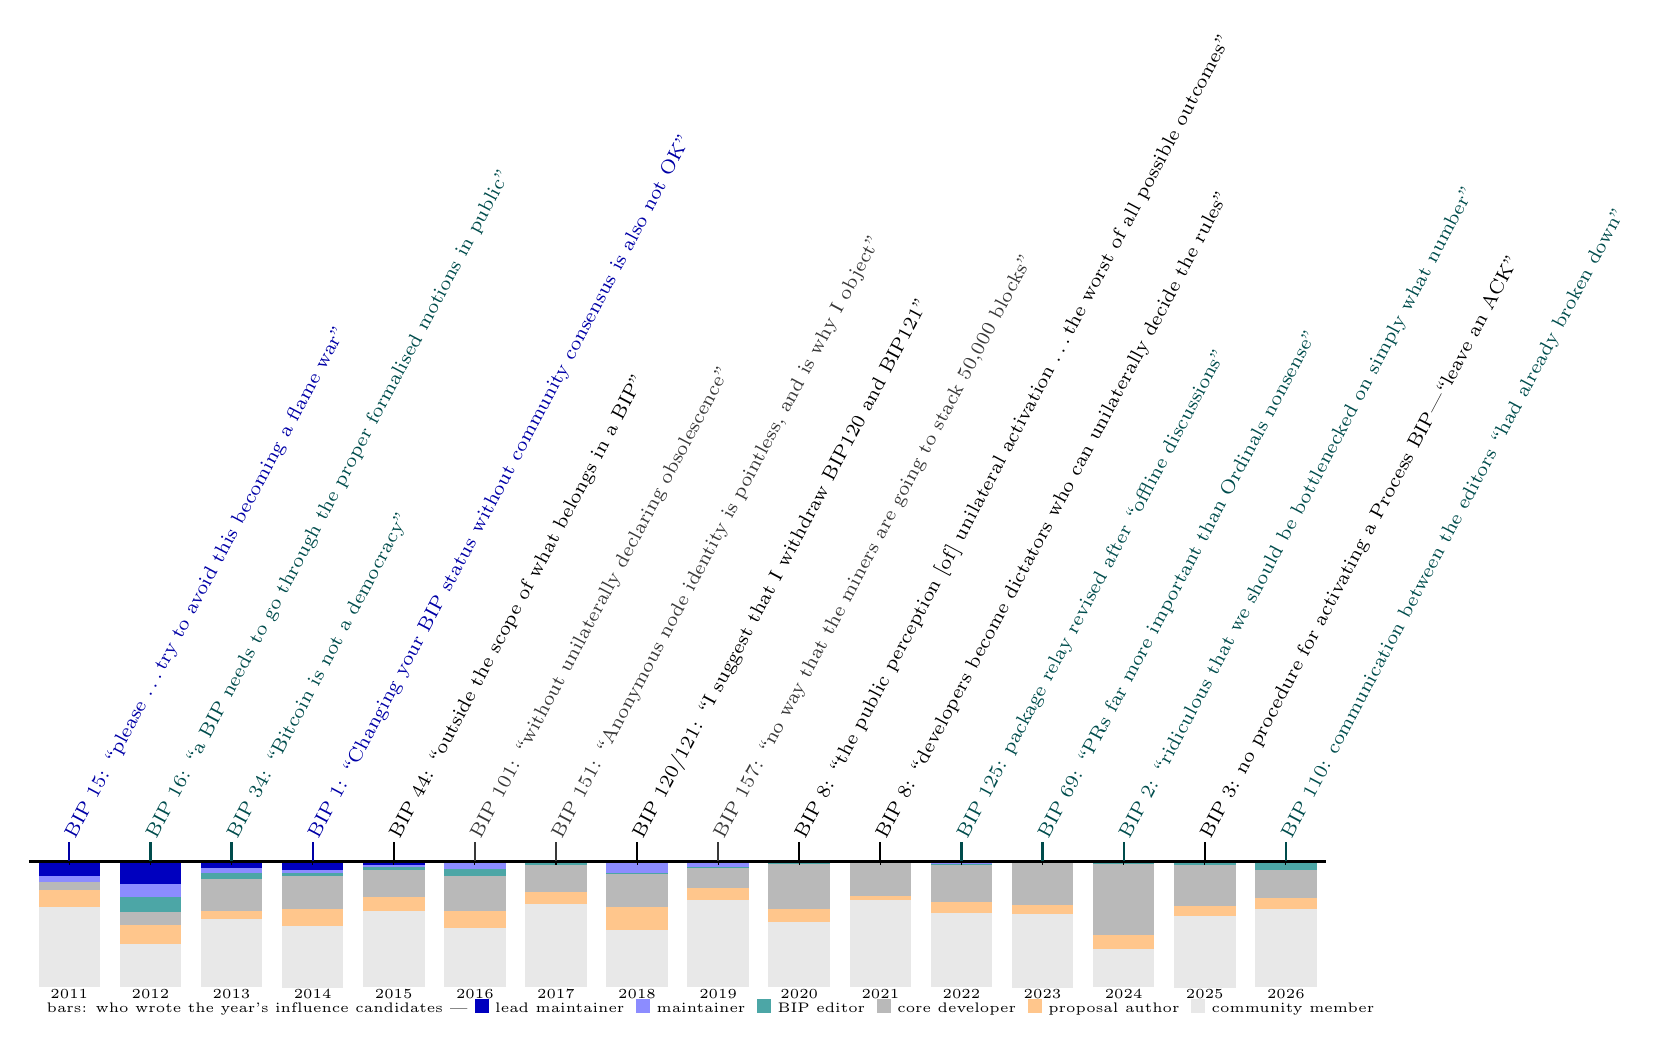
\begin{tikzpicture}[x=1.03cm, y=1cm, font=\scriptsize]
  % stacked role shares per year: lead maintainer, maintainer, BIP editor, core developer, proposal author, community
  \foreach \yr/\a/\b/\c/\d/\e/\f in {
    2011/11.7/4.4/0.0/6.3/13.6/64.0, 2012/17.8/10.8/11.8/9.7/15.1/34.8, 2013/5.4/3.7/4.6/25.3/6.7/54.3,
    2014/6.6/2.5/2.2/26.1/14.1/48.7, 2015/2.7/1.8/2.3/21.2/11.5/60.5, 2016/0.0/6.1/5.1/28.4/13.5/46.9,
    2017/0.0/0.8/2.2/21.3/9.4/66.3, 2018/0.0/9.5/0.5/25.9/18.5/45.6, 2019/0.0/4.7/0.5/15.9/9.2/69.7,
    2020/0.0/0.1/1.6/35.9/10.6/51.8, 2021/0.0/0.0/1.4/26.1/3.5/69.0, 2022/0.0/2.0/1.0/29.5/8.2/59.3,
    2023/0.0/0.8/0.4/33.1/7.8/58.0, 2024/0.0/0.7/1.7/56.2/10.8/30.5, 2025/0.0/0.2/2.5/32.3/8.0/57.1,
    2026/0.0/0.0/6.9/22.0/8.7/62.4} {
    \pgfmathsetmacro{\xl}{\yr-2011+0.12}
    \pgfmathsetmacro{\xr}{\yr-2011+0.88}
    \pgfmathsetmacro{\ya}{-\a*0.016}
    \pgfmathsetmacro{\yb}{\ya-\b*0.016}
    \pgfmathsetmacro{\yc}{\yb-\c*0.016}
    \pgfmathsetmacro{\yd}{\yc-\d*0.016}
    \pgfmathsetmacro{\ye}{\yd-\e*0.016}
    \pgfmathsetmacro{\yf}{\ye-\f*0.016}
    \fill[blue!75!black] (\xl,0) rectangle (\xr,\ya);
    \fill[blue!45] (\xl,\ya) rectangle (\xr,\yb);
    \fill[teal!70] (\xl,\yb) rectangle (\xr,\yc);
    \fill[gray!55] (\xl,\yc) rectangle (\xr,\yd);
    \fill[orange!45] (\xl,\yd) rectangle (\xr,\ye);
    \fill[gray!18] (\xl,\ye) rectangle (\xr,\yf);
  }
  \node[anchor=west, font=\tiny, align=left] at (0.1,-1.85) {bars: who wrote the year's influence candidates ---
    \textcolor{blue!75!black}{\rule{5pt}{5pt}} lead maintainer\;
    \textcolor{blue!45}{\rule{5pt}{5pt}} maintainer\;
    \textcolor{teal!70}{\rule{5pt}{5pt}} BIP editor\;
    \textcolor{gray!55}{\rule{5pt}{5pt}} core developer\;
    \textcolor{orange!45}{\rule{5pt}{5pt}} proposal author\;
    \textcolor{gray!18}{\rule{5pt}{5pt}} community member};
  \draw[thick] (0,0) -- (16,0);
  \foreach \yr in {2011,2012,...,2026} {
    \draw (\yr-2011+0.5,0.05) -- (\yr-2011+0.5,-0.05);
    \node[font=\tiny] at (\yr-2011+0.5,-1.68) {\yr};
  }
  \tikzset{lead/.style={blue!65!black}, ed/.style={teal!60!black}, dev/.style={black}, com/.style={gray!45!black}}
  \foreach \yr/\c/\t in {
    2011/lead/{BIP 15: ``please \ldots try to avoid this becoming a flame war''},
    2012/ed/{BIP 16: ``a BIP needs to go through the proper formalised motions in public''},
    2013/ed/{BIP 34: ``Bitcoin is not a democracy''},
    2014/lead/{BIP 1: ``Changing your BIP status without community consensus is also not OK''},
    2015/dev/{BIP 44: ``outside the scope of what belongs in a BIP''},
    2016/com/{BIP 101: ``without unilaterally declaring obsolescence''},
    2017/com/{BIP 151: ``Anonymous node identity is pointless, and is why I object''},
    2018/dev/{BIP 120/121: ``I suggest that I withdraw BIP120 and BIP121''},
    2019/com/{BIP 157: ``no way that the miners are going to stack 50,000 blocks''},
    2020/dev/{BIP 8: ``the public perception [of] unilateral activation \ldots the worst of all possible outcomes''},
    2021/dev/{BIP 8: ``developers become dictators who can unilaterally decide the rules''},
    2022/ed/{BIP 125: package relay revised after ``offline discussions''},
    2023/ed/{BIP 69: ``PRs far more important than Ordinals nonsense''},
    2024/ed/{BIP 2: ``ridiculous that we should be bottlenecked on simply what number''},
    2025/dev/{BIP 3: no procedure for activating a Process BIP---``leave an ACK''},
    2026/ed/{BIP 110: communication between the editors ``had already broken down''}} {
    \draw[\c, thick] (\yr-2011+0.5,0) -- (\yr-2011+0.5,0.25);
    \node[\c, rotate=62, anchor=west, inner sep=1pt] at (\yr-2011+0.5,0.27) {\t};
  }
\end{tikzpicture}
\caption{Landmark influence acts nominated by Influence Miner for Bitcoin, 2011--2026: for each year, the highest-scoring sentence carrying a controversial mechanism, coloured by the writer's role (dark blue: lead maintainer; teal: maintainer or BIP editor; black: core developer or proposal author; grey: community member); full sentences in Table~\ref{tab:landmarks}. Below the axis, the share of each year's influence candidates written by each role.}
\label{fig:timeline2}
\Description{A horizontal timeline from 2011 to 2026 with one short quoted sentence per year rising from the axis at an angle, and stacked bars below the axis showing the share of influence candidates written by each role per year; the lead maintainer's share disappears after 2015 and core developers' share grows.}
\end{figure*}

\begin{table*}[t]
\caption{The landmark influence acts of Figure~\ref{fig:timeline2}: for each year, the highest-scoring sentence carrying a controversial mechanism (score in brackets; mechanisms as labelled by the tool).}
\label{tab:landmarks}
\footnotesize
\begin{tabular}{p{0.03\textwidth}p{0.05\textwidth}p{0.15\textwidth}p{0.11\textwidth}p{0.58\textwidth}}
\toprule
Year & BIP & Author (role) & Mechanisms & Sentence \\
\midrule
2011 & 15 & Andresen (lead maint.) & tactical, incivility & First: everybody please try to focus on the issues/ideas, and try to avoid this becoming a flame war. [2.2] \\
2012 & 16 & Taaki (BIP editor) & procedural & My feeling is that a BIP needs to go through the proper formalised motions in public before becoming accepted. [3.3] \\
2013 & 34 & Maxwell (BIP editor) & unilateral & Bitcoin is not a democracy---it quite intentionally uses the consensus mechanism only for the one thing that nodes can not autonomously and interdependently validate (the ordering of transactions). [1.9] \\
2014 & 1 & van der Laan (lead maint.) & coalition, backchannel & Changing your BIP status without community consensus is also not OK. [3.0] \\
2015 & 44 & Dashjr (core dev.) & standards, procedural & Things which only improve altcoins, while a perfectly fine thing to standardise, are outside the scope of what belongs in a BIP. [3.4] \\
2016 & 101 & Bishop (community) & ecosystem, unilateral & Nothing about this should be an ``emergency'', we have all the time in the world to prepare a safe and responsible way to upgrade the network without unilaterally declaring obsolescence. [2.9] \\
2017 & 151 & Voskuil (community) & strategic, gatekeeping & Anonymous node identity is pointless, and is why I object to BIP151. [3.0] \\
2018 & 120 & Rosenbaum (author) & exit threat & If there is no good solution to the soft-fork issue, I suggest that I withdraw BIP120 and BIP121. [4.0] \\
2019 & 157 & Moral Agent (community) & ecosystem, economic, gatekeeping & There is no way that the miners are going to stack 50,000 blocks on top of an invalid block without the economic majority abandoning the invalid chain. [2.3] \\
2020 & 8 & Corallo (core dev.) & operational, unilateral & To not make every attempt to distance the activation method from the public perception unilateral activation strikes me as the worst of all possible outcomes for Bitcoin's longevity. [2.5] \\
2021 & 8 & Tim\'on (core dev.) & authority, ecosystem, unilateral & Most devs perceive that not giving miners veto power over proposals somehow means that then developers become dictators who can unilaterally decide the rules. [3.1] \\
2022 & 125 & Zhao (maintainer) & operational, ecosystem, backchannel & I've made some significant changes to my package relay proposal based on observations while implementing, feedback on this thread, and offline discussions. [3.0] \\
2023 & 69 & Dashjr (BIP editor) & incivility & There are several PRs far more important than Ordinals nonsense that need to be triaged and probably merged. [2.5] \\
2024 & 2 & Chow (maintainer) & incivility & It's ridiculous that we should be bottlenecked on simply what number a proposal should have. [3.2] \\
2025 & 3 & Erhardt (author) & procedural & Since BIP 2 doesn't specify a procedure for activating Process BIPs, I suggest that people who wish to state their support leave an ACK on \#1820 or reply in this thread. [3.9] \\
2026 & 110 & Erhardt (BIP editor) & authority, ecosystem, backchannel & Communication between Luke and other BIP Editors had already broken down last year, following a discussion about his attempt to side-step the process by prematurely assigning a BIP number out of band. [3.1] \\
\bottomrule
\end{tabular}
\end{table*}

\subsection{The Three BIPs of the Earlier Study}
\label{sec:icis}

The group's earlier Bitcoin study \cite{thapa2021bitcoin} examined three rule changes by hand: the activation mechanism BIP~9, Segregated Witness (BIP~141) and Taproot (BIPs 340--342). It identified the ``influencers'' of each discussion by social-network centrality on the mailing-list threads and, by reading the threads, IRC meeting minutes and podcasts, described five tactics through which those influencers steered the decisions, derived from the lateral-influence tactics of Ngwenyama and Nielsen \cite{ngwenyama2014} (rational persuasion, personal appeals, reciprocity, alliance, intermediaries): \emph{political neutrality} (T1: the influencer favours Bitcoin as a whole, not a faction), \emph{shepherding the community} (T2: identifying issues and laying out the steps to resolve them), a \emph{participative approach} (T3: seeking input and using it to form an alliance), \emph{sticking to the laid plan} (T4: holding the community to an agreement already made) and \emph{developing reciprocal relationships} (T5: deals between member groups, such as the Hong Kong and New York agreements). Table~\ref{tab:icis} maps those tactics onto the mechanisms Influence Miner labels, and Table~\ref{tab:icisbips} gives the tool's profile of the same three discussions over their whole life, including the years after the earlier study closed.

\begin{table}[t]
\caption{The five influencer tactics of the earlier Bitcoin study \cite{thapa2021bitcoin} and the Influence Miner mechanisms that carry them.}
\label{tab:icis}
\footnotesize
\begin{tabular}{p{0.30\columnwidth}p{0.62\columnwidth}}
\toprule
Tactic (source of influence) & Mechanisms in which it surfaces \\
\midrule
T1 Political neutrality (personal appeals, rational persuasion) & \emph{strategic} (the long-term good of Bitcoin, decentralisation, censorship resistance); \emph{user demand} (``real users'', ``the ecosystem'') \\
T2 Shepherding the community (identification, development, evaluation) & \emph{tactical} (summarising, reframing, ``the real question is''), \emph{operational} (laying out implementation and deployment steps), \emph{security} and \emph{compatibility} (naming the risks to be resolved) \\
T3 Participative approach (alliance) & \emph{coalition} (``several people'', ``consensus seems to be''), \emph{user demand}; and, when the alliance is with companies or miners, \emph{organizational} and \emph{corporate interest} \\
T4 Stick to the laid plan (personal appeals, solution evaluation) & \emph{procedural control} (``that's not how BIP 9 works'', ``out of scope''), \emph{gatekeeping} (refusals to reopen a settled question), \emph{standards} (``as the BIP says'') \\
T5 Developing reciprocal relationships (reciprocity) & \emph{backchannel} (agreements reached off-list, at conferences, on IRC), \emph{organizational} and \emph{economic} (what miners, companies and exchanges get in return) \\
\bottomrule
\end{tabular}
\end{table}

\begin{table}[t]
\caption{Influence Miner's profile of the three discussions of the earlier study (\% of the BIP's candidates; whole life of the discussion).}
\label{tab:icisbips}
\footnotesize
\setlength{\tabcolsep}{3.5pt}
\begin{tabular}{lrrrr}
\toprule
 & BIP 9 & BIP 141 & BIP 340/341 & BIP 342 \\
\midrule
Candidates & 3,065 & 2,598 & 3,261 & 551 \\
Participants & 107 & 97 & 98 & 29 \\
Years & 2015--26 & 2016--26 & 2020--26 & 2020--26 \\
\midrule
Ecosystem & 36.1 & 39.8 & 22.6 & 16.2 \\
Operational & 40.9 & 24.7 & 20.1 & 21.4 \\
Compatibility & 22.2 & 16.1 & 8.0 & 11.4 \\
Security & 12.1 & 14.4 & 27.0 & 12.5 \\
Economic & 11.4 & 19.5 & 15.4 & 27.2 \\
Functional & 5.2 & 4.8 & 8.6 & 15.1 \\
Strategic & 2.2 & 2.8 & 7.5 & 10.2 \\
Tactical & 3.3 & 2.9 & 3.9 & 2.7 \\
Coalition & 2.7 & 2.1 & 2.1 & 1.8 \\
Authority & 2.5 & 1.2 & 1.3 & 1.1 \\
Any controversial & 2.7 & 2.6 & 3.8 & 2.0 \\
\bottomrule
\end{tabular}
\end{table}

The profiles agree with the earlier reading and add to it. BIP~9 and BIP~141 are the two most \emph{operational} and \emph{compatibility}-laden discussions in the corpus (40.9\% and 22.2\% for BIP~9): they were argued as questions of how to activate a rule and what would happen to nodes and miners that did not follow, which is the substance of the shepherding and stick-to-the-plan tactics the earlier study found there. Taproot, by contrast, is the most \emph{security}-laden (27\%) and \emph{strategic} (7.5\%) discussion---the cryptographic design was argued on attack surface and on Bitcoin's long-term direction, the register of political neutrality---and it is the only one of the three with a controversial share above the corpus average, most of it from the 2021 activation dispute rather than from the design. The tool also names the people the earlier study had to anonymise: on BIP~9 the most active participants were Johnson Lau, Jorge Tim\'on, Anthony Towns, shaolinfry, Matt Corallo and Ariel Luaces; on BIP~141 Johnson Lau (as author), Gloria Zhao, Antoine Riard, James Hilliard, Eric Voskuil and Matt Corallo---with Zhao's and Riard's contributions coming after 2021, in the package-relay and mempool-policy threads that reference SegWit; on BIP~341 Antoine Riard, Anthony Towns (as author), \emph{conduition}, Yuval Kogman, Salvatore Ingala and James T. None of the six most active participants on any of the three BIPs is a maintainer or an editor, which is the earlier study's finding about ``influencers'' without formal office, measured a different way. What the sentence-level labels add is the content of the influence: the earlier study described the influencers' \emph{manner} (neutral, participative, plan-bound); the mechanisms describe the \emph{arguments}, and show that the manner rode on operational, compatibility and ecosystem claims for the activation debates and on security and strategic claims for Taproot. What they cannot add is the reciprocity tactic: deals between companies and miners were made in Hong Kong and New York, not on the list, and the tool sees only their traces (``as was discussed at the summit'', ``the position of Blockstream employees'').

\section{Bitcoin and Python Compared}
\label{sec:compare}

The Python study designed the comparison this paper completes. Table~\ref{tab:compare} sets the two projects side by side on the same detector, using Python's extended corpus (1999--2026, 299,192 candidates) and Bitcoin's (2011--2026, 62,791 candidates).

\begin{table}[t]
\caption{Bitcoin and Python on the same instrument (\% of candidates unless stated).}
\label{tab:compare}
\small
\setlength{\tabcolsep}{4pt}
\begin{tabular}{lrr}
\toprule
 & Bitcoin & Python \\
\midrule
Proposals with candidates & 199 & 764 \\
Candidate sentences & 62,791 & 299,192 \\
Participants & 636 & 3,639 \\
Mechanisms per candidate & 1.38 & 1.27 \\
\midrule
Ecosystem & 33.7 & 18.4 \\
Operational & 22.0 & 27.0 \\
Security & 17.5 & 2.6 \\
Economic & 14.8 & 2.3 \\
Compatibility & 12.1 & 13.6 \\
Functional & 7.6 & 25.8 \\
Standards & 6.5 & 8.8 \\
Organizational & 4.5 & 3.2 \\
Strategic & 4.2 & 5.0 \\
Tactical & 3.3 & 4.9 \\
User demand & 3.1 & 3.6 \\
Authority & 2.5 & 7.6 \\
Coalition & 2.1 & 2.0 \\
\midrule
Supporting / blocking / revising & 1.5 / 1.4 / 8.7 & 2.0 / 1.5 / 8.8 \\
External or mixed scope & 27.6 & 7.7 \\
Formal leader's share of candidates$^a$ & 1.0 & 8.0 \\
Community members' share & 57.6 & 37.1 \\
Any controversial mechanism & 3.9 & 4.7 \\
Supporting aligned with outcome & 74.9 & 70.0 \\
Blocking aligned with outcome & 12.1 & 26.5 \\
\bottomrule
\multicolumn{3}{l}{\footnotesize $^a$ lead maintainer (Bitcoin); BDFL plus Steering Council (Python).}
\end{tabular}
\end{table}

\paragraph{What the taxonomy predicted.} The Python paper expected Bitcoin to show stronger ecosystem, economic, security and deployment-based influence and weaker internal role-based influence. All four expectations hold, and by large margins: ecosystem signals are 1.8 times as frequent, security 6.7 times, economic 6.3 times, and authority a third as frequent. Scope confirms the same picture from another angle: 27.6\% of Bitcoin's candidates name external constituencies---users, wallets, exchanges, miners, companies---against 7.7\% in Python. Bitcoin's arguments are about the world outside the repository because the world outside the repository decides.

\paragraph{What it did not predict.} Three differences were not anticipated. First, \emph{functional} argument---whether the design solves the problem---is Python's second mechanism (25.8\%) and Bitcoin's sixth (7.6\%). Python's discussions are about language design, where the question is whether a feature is worth having; Bitcoin's are about protocol changes, where the question of whether a change is desirable is settled quickly and the argument moves to whether it is safe, what it costs and who will run it. Second, the formal leader is nearly absent from Bitcoin's record. Python's BDFL wrote 8\% of candidates and pronounced on most contested PEPs; Bitcoin's lead maintainers wrote 1\% and, after 2015, nothing that the tool counts as argument. The lead maintainer role in Bitcoin was administrative---merge, release, announce---and its holders declined to argue proposals on the list, which is why the era comparison shows no analogue of Python's authority-invoking council. Third, the Python paper's temporal finding---signalling peaking in the four weeks around the decision---does not transfer, for a reason that is itself a finding about governance: in Bitcoin the repository's status change records a deployment, not a decision, and the decision is distributed across merges, releases, signalling periods and node upgrades that no single timestamp captures.

\paragraph{What is the same.} Direction distributions are nearly identical (about 88\% neutral, 9\% revising, 1.5\% supporting, 1.4\% blocking), stance alignment with outcomes sits at the base rate in both projects, coalition signals are equally rare (2\%), and controversial mechanisms mark about one candidate in twenty-five in Bitcoin and one in twenty in Python. Two communities with opposite governance designs---a single decision-maker replaced by a council, and no decision-maker at all---argue with the same explicitness and the same small share of contested moves; what differs is what they argue about and who does the arguing.

\section{Discussion}

\paragraph{What the mechanism profile says about Bitcoin.} Bitcoin's proposal discussions are dominated by arguments about the ecosystem, about deployment, about attacks and about incentives. This is the profile of a community whose changes are adopted by third parties rather than shipped by the project: a change must be safe for the nodes that will run it, affordable for the miners and users who will pay for it, and acceptable to the wallets and exchanges that will implement it, and every one of those constituencies can refuse. Authority is rarely invoked because there is little to invoke; the BIP editors administer numbers, the maintainers merge code, and the lead maintainers---while they existed---did not argue. The mechanism the Python paper called \emph{functional}, the argument about whether a proposal is a good idea, is where Python spends a quarter of its influence and Bitcoin a thirteenth: Bitcoin's proposals are less often bad ideas than dangerous or expensive ones.

\paragraph{Governance without a governor.} The era comparison shows what governance looks like when it is contested rather than delegated. The block-size war has the highest compatibility share of any period and a fall in controversial mechanisms rather than a rise; the community argued the war as a compatibility question and, on this measure, argued it more civilly than it argued the early BIPs or the post-lead debates. The post-lead era shows a different signature: security and economic arguments at their peak, the formal roles almost silent, core developers writing a third of all candidates, and controversial mechanisms rising again---driven, as Section~\ref{sec:rq6} shows, by incivility and procedural control around the covenant proposals, the relay-policy disputes and the editorship itself. In Python the transition from a person to a council moved contested influence from fiat to process; in Bitcoin the disappearance of the lead maintainer moved it from a small formal core to a larger informal one, and the process questions that Python's council absorbed are fought on the list.

\paragraph{The decision is not in the repository.} The most consequential methodological result is the failure of the decision-window analysis to transfer. Influence Miner's temporal features assume that a proposal has a decision date; Python's PEP repository supplies one because the BDFL's pronouncement and the status change coincide. Bitcoin's repository supplies a deployment date, often years later and sometimes in bulk. A tool that wants to find the decision in Bitcoin must look elsewhere: at the merge of the implementation, the release that ships it, the start and end of the signalling period, the flag day. The state history built here from the \texttt{bitcoin/bips} repository is the wrong clock for that question, and future work should assemble the right one from the reference implementation's release history and the activation records on the chain.

\paragraph{Volume is not influence, again.} Stance alignment sits at the base rate in Bitcoin as in Python, and the blocking figure is lower still because Bitcoin rarely rejects a BIP formally---contested proposals stay drafts. A decision-mining tool that counted objections would conclude that objections never work; the record of BIP 101, BIP 148 and BIP 119 says otherwise. The mechanisms and roles attached to each sentence are what let an analyst see that the objections that stopped the block-size increase were compatibility and ecosystem arguments from developers, and that the objections that stalled the covenant proposals were security and economic arguments from the community.

\paragraph{Corpus building as a contribution.} The Bitcoin corpus took one working day to build from three public sources, and the same scripts will rebuild it next year. Two of its properties deserve emphasis for other researchers: the public-inbox mirror is the only archive that spans all three homes of the list, and the Google Groups era is unusable without recovering the original sender from \texttt{X-Original-From}. The BIP repository's 2025 relabelling, which collapsed rejected, withdrawn and obsolete proposals into ``Closed'', is a warning that a proposal repository's current state can erase the distinctions a study needs; the git history keeps them.

\section{Data-Quality Findings in the Bitcoin Corpus}
\label{sec:dataquality}

Four properties of the sources would have distorted the results if left untreated. \emph{Release announcements}: the lead maintainer's release notes list every BIP shipped in a release; the announcement of Bitcoin Core 0.21.0 alone produced 1,557 candidate sentences on a first run, and van der Laan appeared as the most influential participant in the corpus. A subject filter now skips the announcements themselves (229 messages) while keeping the replies. \emph{DMARC rewriting}: Google Groups replaces the sender address of every post with the group's own; 687 messages would have been credited to one ``sender'' called \emph{conduition}, the display name of the first such post the loader saw. \emph{Bulk status changes}: 143 of the 505 status changes in the BIP repository happened on 12 April 2025, and 48 more on four other days, so a decision date read naively from the history is often the date of a clean-up. \emph{Technical homonyms}: Bitcoin's vocabulary collides with the controversial cue lists in ways Python's does not---\emph{unilateral} (Lightning's unilateral close), \emph{fork off} and \emph{split the chain} (protocol behaviour), \emph{offline} and \emph{out of band} (wallets and signing), \emph{funds paid to} (outputs), \emph{dumb} (dumb clients). Four passes over the full corpus were needed to add the disambiguating contexts, and the residual inflation of \emph{backchannel} and \emph{ecosystem} by technical uses is noted where it matters.

\section{Threats to Validity}
\label{sec:threats}

\paragraph{Construct validity.} The labels are cue-based and unvalidated; the sample tables show that the cues catch what they were written for and also that they catch technical homonyms. The base mechanisms most affected are \emph{ecosystem} (nodes, wallets and miners as components) and \emph{security} (attack as a protocol term); the rank order of mechanisms is robust to this, the absolute shares are not. The stratified annotation sample that the tool exports is the instrument for the two-coder study.

\paragraph{Coverage.} Only messages that name a BIP number are linked. Proposals are discussed by name before they have a number (``Taproot'', ``CTV'', ``the block size'') and many threads on bitcoin-dev never mention a BIP at all; 6,886 of 24,391 messages are linked. The pre-number phase of a proposal is therefore under-represented, which contributes to the small early-discussion share in RQ1. Title matching, as used in the earlier DeMaP Miner study of BIPs, would raise coverage and is the first extension to make.

\paragraph{Roles.} Rosters were derived from the repositories: maintainers from merge commits (which since 2021 are made by a bot on maintainers' behalf, so recent terms were set open-ended by hand), core developers from a commit threshold, editors and lead maintainers from documented terms. People are matched by clustered display name; pseudonymous participants who changed handles are counted twice. Companies are not resolved: the corporate-interest mechanism sees what people say about employers, not who employs them.

\paragraph{External validity.} The corpus is one mailing list. Bitcoin's decisions are also made on GitHub pull requests, on IRC (whose logs the earlier study used) and, since 2024, on Delving Bitcoin; the list carries the proposal announcements and the set-piece debates, not the code review. Findings are about how influence is exercised where BIPs are discussed publicly.

\section{Conclusion}

This paper applied Influence Miner to the complete public record of Bitcoin's proposal discussions, after rebuilding the corpus from the public-inbox mirror of bitcoin-dev, the BIP repository's history and the reference implementation's commit history. Across 199 BIPs and 62,791 candidate sentences, Bitcoin argues about the ecosystem, deployment, security and incentives where Python argues about implementation and design; its formal leaders barely argue at all; its decisions are recorded by the repository long after they are taken; its most contested period was argued as a compatibility question; and its controversial influence has shifted, since the lead maintainer left, from the formal core to a larger informal one and from fiat to process and incivility. Measured on the same instrument, the two projects differ in what they argue about and who argues, and agree in how explicitly they argue and how little stance volume tells about outcomes. The next steps are the annotation study, title-based linking of pre-number discussions, a decision clock built from releases and activations rather than repository status, the Preference Miner run that RQ5 needs, and the extension of the corpus to the pull-request and Delving Bitcoin venues.

\appendix

\section{Detector Rules}
\label{app:rules}

The rules are reproduced here so that the labels in this paper can be reproduced and criticised. All cues are matched case-insensitively on word boundaries; British and American spellings are both listed.

\paragraph{Mechanism cues (selection).} Table~\ref{tab:cues} lists representative cues per mechanism; the complete lists (about 60 cues per mechanism) are in \texttt{InfluenceTypeDetector.java}. Some broad words count only near a disambiguating word within 60 characters: \emph{break/breaks/broken} near \emph{compatib-, existing, code, API, user, change, backward}; \emph{risk} near \emph{security, attack, regression, break, compat, data, safety}; \emph{team} near \emph{release, core, dev, steering, security}; \emph{node(s)} near \emph{old, full, network, bitcoin, upgrade}; \emph{market} near \emph{fee, share, economic, incentive}; \emph{patch(es)} near \emph{submit, review, apply, reference, implement}; \emph{editor(s)} near \emph{PEP, BIP}; \emph{data} near \emph{show, evidence, measure, benchmark}. The word \emph{safe} on its own is not a cue. The controversial mechanisms are matched the same way, and their broad cues also need context: ownership claims (\emph{I maintain, my module, as the maintainer}) count only near a refusal or decision word; \emph{no way, no chance, won't happen} only near a proposal or refusal word; \emph{offline, in person, at PyCon, at the sprint} only near a discussion or decision word; \emph{internally, secret} only near deliberation words; \emph{grant, contract, hired, full-time} only near employer or funding words; \emph{exhausted, tired of, step down, walk away, hiatus, retire} only in the first person or near a project word; \emph{angry, insane, flame, insult, hostile} only next to a person or tone word; \emph{procedure, belongs on, the archives, drop it, please stop} only near a process, list or thread word. For Bitcoin the lists were extended with the vocabulary of its governance: \emph{lead maintainer, core maintainer(s), BIP editors, wladimir, gavin, gmaxwell, sipa} (authority); the companies and funders active in the project---\emph{at Blockstream/Chaincode/Coinbase/Bitmain/BitPay/Square/Spiral/Brink/MIT DCI/Lightning Labs}, \emph{pays my salary, grant from, OpenSats}---(corporate interest); \emph{fork bitcoin, contentious hard fork, split the chain, run Bitcoin XT/Classic/Unlimited, leave bitcoin, sell my coins} (exit threat); \emph{censored, censoring, banned from the list, moderation queue, list moderators, this is bitcoin-dev, not} (procedural control); and \emph{shill, scam, sockpuppet, brigading, concern troll, bad faith, dishonest, disingenuous} (incivility).

\begin{table*}[t]
\caption{Representative cue phrases per mechanism (base mechanisms above the rule, controversial mechanisms below).}
\label{tab:cues}
\small
\begin{tabular}{p{0.15\textwidth}p{0.81\textwidth}}
\toprule
Mechanism & Cues \\
\midrule
Strategic & long term, future direction, philosophy, principles, Zen of Python, pythonic, readability, simplicity, decentrali[s/z]ation, project values, governance \\
Operational & implement(ation), maintain(ance), release, migration, deploy(ment), test suite, documentation, backport, feature freeze, reference implementation, CPython \\
Functional & solves, use case, edge case, corner case, API, behavio[u]r, semantics, syntax, alternative design, better approach, what problem, special case \\
Tactical & to summari[s/z]e, let's decide, can we agree, compromise, reframe, narrow, clarify, evidence, defer, postpone, next step, rough consensus, separate PEP, straw poll \\
Authority & BDFL, steering council, delegate, core developer(s), committer, maintainer, BIP editor, release manager, pronounce(ment), veto, Guido, final decision \\
Compatibility & backward(s) compatib-, incompatible, breaking change, existing code/users, legacy, Python 2/3, 2to3, deprecat-, regression, soft/hard fork \\
Security & security, attack(er), vulnerab-, risk, unsafe, safety, privacy, robust(ness), denial of service, exploit, double spend, consensus failure, crash, data loss \\
Standards & standard(s), specification, spec, RFC, convention, interoperab-, compliance, PEP~8, style guide, de facto standard \\
Ecosystem & ecosystem, downstream, librar(y/ies), package(s), PyPI, stdlib, third-party, distros, wallet(s), exchange(s), miner(s), node(s), Lightning, full node \\
Economic & cost(s), expensive, funding, incentive(s), fee(s), fee market, business, commercial, budget, developer time, block reward, mempool \\
Organizational & company, foundation, PSF, organi[s/z]ation, working group, release team, committee, sponsor, employer, Google, Microsoft, Red Hat, Bitcoin Core \\
Coalition & several/many people, we all agree, consensus seems/is, broad support, multiple developers, as others have said, unanimous(ly), seconded, me too \\
User demand & users want/need, people keep asking, frequently requested, pain point, beginners, newcomers, students, real users, widely used, adoption \\
\midrule
Unilateral & I have decided, I'm going to reject/accept, I hereby, consider it accepted, end of discussion, not up for debate, overrule, by fiat, pull rank, already merged/committed, as BDFL, BDFL pronouncement, I get to decide, made up my mind \\
Corporate interest & my employer, my/our company, at work, at Google/Dropbox/Microsoft/Red Hat/\ldots, our production, our customers, paid to, funded by, sponsored by, commercial interest, business needs, conflict of interest, internal fork, enterprise users, my manager \\
Gatekeeping & I will not merge, I won't accept, not going to happen, over my dead body, I refuse, I will revert, I veto, I (strongly) object, not on my watch, as the maintainer, my approval, dead on arrival, won't fly, no chance, $-$1000, strong $-$1, the answer is no \\
Exit threat & I'll fork, fork CPython, leaving python-dev, I quit, I resign, step down, count me out, I give up, walk away, stop contributing/maintaining, withdraw the PEP, if this goes in, burned out, fed up, last straw, ultimatum, unsubscribe, mute this thread, fight so hard, out of energy \\
Incivility & stupid, idiot, ridiculous, absurd, nonsense, clueless, garbage, shut up, troll, flame war, you (clearly) don't understand, waste of time, bikeshedding, ad hominem, personal attack, insult, rude, hostile, toxic, condescending, arrogant, harassment, code of conduct, calm down, who cares \\
Backchannel & offline, off-list, privately, in private, behind closed doors, at the sprint, language summit, at PyCon, on IRC/Zulip/Discord, I talked to, Guido and I, Guido told me, already been decided, without discussion, without consulting, python-committers, done deal, rubber stamp, cabal, inner circle, out of band, lack of transparency \\
Procedural control & wrong list/venue, belongs on python-ideas, take it to, out of scope, scope creep, PEP~1 says, the PEP process, follow the process, proper channels, moderator, locking this thread, please stop, drop it, already discussed, dead horse, read the archives, needs a sponsor, write a PEP, too late for, after the freeze, PEP~13, formal vote \\
\bottomrule
\end{tabular}
\end{table*}

\paragraph{Direction.} A sentence is \emph{supporting} on an explicit support phrase or a positive vote (\emph{+1, +0.5} at a token boundary), \emph{blocking} on an explicit objection or a negative vote (\emph{$-$1}); negated phrases are resolved first (\emph{I don't object, no objection, not against, can live with} $\rightarrow$ supporting; \emph{don't support, not in favour, not convinced, don't see the need, not worth} $\rightarrow$ blocking); a sentence with both supporting and blocking cues is ambiguous and stays \emph{neutral}; hedged sentences (\emph{maybe, perhaps, not sure, I wonder}) and questions never become supporting or blocking and are demoted to \emph{revising} when they carry a stance cue; otherwise \emph{revising} on revision cues (\emph{revise, alternative, compromise, defer, postpone, clarify, narrow the scope, needs more work, more evidence, instead of, what about, I'd prefer, unless, provided that}) and \emph{neutral} by default.

\paragraph{Scope and target.} Scope is \emph{internal} when the author's resolved role is one of BDFL, steering council, delegate, proposal author, PEP/BIP editor, core developer, release manager or maintainer, or when the sentence names such actors; \emph{external} when the sentence names users, downstream projects, libraries, companies, wallets, exchanges, miners, standards bodies, educators, researchers or ``my employer''; \emph{mixed} when both apply. The role alone never makes a sentence external. Target is the first of governance, security, compatibility, implementation, ecosystem, users and proposal whose cue list matches.

\paragraph{Preprocessing.} Lines are dropped when they start with a quote marker, are ``On \ldots wrote:'' introductions, mail headers, forwarded-message markers, message-id or address debris, Gmail-style dated quote introductions, divider lines, signature blocks (from ``\texttt{--}'' or a closing word such as \emph{regards, cheers, thanks} to the end unless prose resumes), mailing-list footers, embedded PEP text (from a ``PEP: \emph{n}'' header block onward), code, diffs or tracebacks. URLs become \texttt{<URL>}. Sentences are split on terminal punctuation followed by whitespace with abbreviations, version numbers and proposal references protected; short vote lines are kept whole; sentences of fewer than three words (other than votes), more than 120 words, or mostly non-alphabetic characters are dropped; duplicates within a proposal are collapsed after lower-casing and removing punctuation.

\begin{thebibliography}{00}

\bibitem{pep1}
Python Software Foundation. 2026. PEP 1 -- PEP Purpose and Guidelines. Retrieved September 12, 2026 from \url{https://peps.python.org/pep-0001/}

\bibitem{pep13}
Python Software Foundation. 2026. PEP 13 -- Python Language Governance. Retrieved September 12, 2026 from \url{https://peps.python.org/pep-0013/}

\bibitem{bitcoinbips}
Bitcoin Core Contributors. 2026. Bitcoin Improvement Proposals repository. Retrieved September 12, 2026 from \url{https://github.com/bitcoin/bips}

\bibitem{bip3}
Bitcoin Core Contributors. 2026. BIP 3 -- Updated BIP Process. Retrieved September 12, 2026 from \url{https://github.com/bitcoin/bips/blob/master/bip-0003.md}

\bibitem{influenceMinerBitcoin}
Pankaj Sharma. 2026. Influence Miner for Bitcoin: How influence is exercised in Bitcoin Improvement Proposal discussions, 2011--2026. Draft manuscript, September 2026.

\bibitem{sharma2021rationale}
Pankajeshwara Nand Sharma, Bastin Tony Roy Savarimuthu, and Nigel Stanger. 2021. Extracting Rationale for Open Source Software Development Decisions -- A Study of Python Email Archives. In \emph{Proceedings of the 43rd IEEE/ACM International Conference on Software Engineering (ICSE 2021)}. IEEE, 1008--1019. \url{https://arxiv.org/abs/2102.05232}

\bibitem{sharma2024rationale}
Pankajeshwara Nand Sharma, Bastin Tony Roy Savarimuthu, and Nigel Stanger. 2024. How are decisions made in open source software communities? Uncovering rationale from Python email repositories. \emph{Journal of Software: Evolution and Process}. \url{https://doi.org/10.1002/smr.2526}

\bibitem{sharma2021roles}
Pankajeshwara Nand Sharma, Bastin Tony Roy Savarimuthu, and Nigel Stanger. 2021. Influence of Roles in Decision-Making during OSS Development -- A Study of Python. \emph{arXiv:2106.02209}. \url{https://arxiv.org/abs/2106.02209}

\bibitem{sharma2022demap}
Pankajeshwara Nand Sharma, Bastin Tony Roy Savarimuthu, and Nigel Stanger. 2022. Unearthing open source decision-making processes: A case study of Python Enhancement Proposals. \emph{Software: Practice and Experience}. \url{https://doi.org/10.1002/spe.3128}

\bibitem{thapa2021bitcoin}
Rewat Thapa, Pankajeshwara Sharma, Joschka Andreas H{\"u}llmann, and Bastin Tony Roy Savarimuthu. 2021. Identifying Influence Mechanisms in Permissionless Blockchain Communities: The Bitcoin Case. In \emph{Proceedings of the 42nd International Conference on Information Systems (ICIS 2021)}, 1--17.

\bibitem{rationaleDesign}
Antony Tang, Yan Jin, and Jun Han. 2007. A rationale-based architecture model for design traceability and reasoning. \emph{Journal of Systems and Software} 80, 6, 918--934.

\bibitem{argumentMining}
Raquel Mochales and Marie-Francine Moens. 2011. Argumentation mining. \emph{Artificial Intelligence and Law} 19, 1, 1--22.

\bibitem{raymond1999}
Eric S. Raymond. 1999. \emph{The Cathedral and the Bazaar: Musings on Linux and Open Source by an Accidental Revolutionary}. O'Reilly.

\bibitem{omahony2007}
Siobh\'an O'Mahony and Fabrizio Ferraro. 2007. The emergence of governance in an open source community. \emph{Academy of Management Journal} 50, 5, 1079--1106.

\bibitem{dahlander2005}
Linus Dahlander and Mats G. Magnusson. 2005. Relationships between open source software companies and communities: Observations from Nordic firms. \emph{Research Policy} 34, 4, 481--493.

\bibitem{riehle2007}
Dirk Riehle. 2007. The economic motivation of open source software: Stakeholder perspectives. \emph{IEEE Computer} 40, 4, 25--32.

\bibitem{zhang2020}
Yuxia Zhang, Minghui Zhou, Klaas-Jan Stol, Jianyu Wu, and Zhi Jin. 2020. How do companies collaborate in open source ecosystems? An empirical study of OpenStack. In \emph{Proceedings of the 42nd International Conference on Software Engineering (ICSE 2020)}, 1196--1208.

\bibitem{ducheneaut2005}
Nicolas Ducheneaut. 2005. Socialization in an open source software community: A socio-technical analysis. \emph{Computer Supported Cooperative Work} 14, 4, 323--368.

\bibitem{jensen2007}
Chris Jensen and Walt Scacchi. 2007. Role migration and advancement processes in OSSD projects: A comparative case study. In \emph{Proceedings of the 29th International Conference on Software Engineering (ICSE 2007)}, 364--374.

\bibitem{hirschman1970}
Albert O. Hirschman. 1970. \emph{Exit, Voice, and Loyalty: Responses to Decline in Firms, Organizations, and States}. Harvard University Press.

\bibitem{robles2012}
Gregorio Robles and Jes\'us M. Gonz\'alez-Barahona. 2012. A comprehensive study of software forks: Dates, reasons and outcomes. In \emph{Open Source Systems: Long-Term Sustainability (OSS 2012)}, IFIP AICT 378, 1--14.

\bibitem{gamalielsson2014}
Jonas Gamalielsson and Bj\"orn Lundell. 2014. Sustainability of open source software communities beyond a fork: How and why has the LibreOffice project evolved? \emph{Journal of Systems and Software} 89, 128--145.

\bibitem{raman2020}
Naveen Raman, Minxuan Cao, Yulia Tsvetkov, Christian K\"astner, and Bogdan Vasilescu. 2020. Stress and burnout in open source: Toward finding, understanding, and mitigating unhealthy interactions. In \emph{ICSE-NIER 2020}, 57--60.

\bibitem{ferreira2021}
Isabella Ferreira, Jinghui Cheng, Bram Adams, and Eirini Kalliamvakou. 2021. The ``shut the f**k up'' phenomenon: Characterizing incivility in open source code review discussions. \emph{Proceedings of the ACM on Human-Computer Interaction} 5, CSCW2, Article 353.

\bibitem{squire2015}
Megan Squire and Rebecca Gazda. 2015. FLOSS as a source for profanity and insults: Collecting the data. In \emph{Proceedings of the 48th Hawaii International Conference on System Sciences (HICSS 2015)}, 5290--5298.

\bibitem{schneider2016}
Daniel Schneider, Scott Spurlock, and Megan Squire. 2016. Differentiating communication styles of leaders on the Linux kernel mailing list. In \emph{Proceedings of the 12th International Symposium on Open Collaboration (OpenSym 2016)}, Article 2.

\bibitem{delaat2007}
Paul B. de Laat. 2007. Governance of open source software: State of the art. \emph{Journal of Management \& Governance} 11, 2, 165--177.

\bibitem{fitzgerald2006}
Brian Fitzgerald. 2006. The transformation of open source software. \emph{MIS Quarterly} 30, 3, 587--598.

\bibitem{transferofpower}
Guido van Rossum. 2018. Transfer of power. Message to python-committers, 12 July 2018. Retrieved September 12, 2026 from \url{https://mail.python.org/pipermail/python-committers/2018-July/005664.html}

\bibitem{mockus2002}
Audris Mockus, Roy T. Fielding, and James D. Herbsleb. 2002. Two case studies of open source software development: Apache and Mozilla. \emph{ACM Transactions on Software Engineering and Methodology} 11, 3, 309--346.

\bibitem{fielding1999}
Roy T. Fielding. 1999. Shared leadership in the Apache project. \emph{Communications of the ACM} 42, 4, 42--43.

\bibitem{crowston2005}
Kevin Crowston and James Howison. 2005. The social structure of free and open source software development. \emph{First Monday} 10, 2.

\bibitem{stewart2005}
Daniel Stewart. 2005. Social status in an open-source community. \emph{American Sociological Review} 70, 5, 823--842.

\bibitem{vonkrogh2003}
Georg von Krogh, Sebastian Spaeth, and Karim R. Lakhani. 2003. Community, joining, and specialization in open source software innovation: A case study. \emph{Research Policy} 32, 7, 1217--1241.

\bibitem{weber2004}
Steven Weber. 2004. \emph{The Success of Open Source}. Harvard University Press.

\bibitem{shah2006}
Sonali K. Shah. 2006. Motivation, governance, and the viability of hybrid forms in open source software development. \emph{Management Science} 52, 7, 1000--1014.

\bibitem{markus2007}
M. Lynne Markus. 2007. The governance of free/open source software projects: Monolithic, multidimensional, or configurational? \emph{Journal of Management \& Governance} 11, 2, 151--163.

\bibitem{dahlander2011}
Linus Dahlander and Siobh\'an O'Mahony. 2011. Progressing to the center: Coordinating project work. \emph{Organization Science} 22, 4, 961--979.

\bibitem{fleming2007}
Lee Fleming and David M. Waguespack. 2007. Brokerage, boundary spanning, and leadership in open innovation communities. \emph{Organization Science} 18, 2, 165--180.

\bibitem{shaikh2017}
Maha Shaikh and Ola Henfridsson. 2017. Governing open source software through coordination processes. \emph{Information and Organization} 27, 2, 116--135.

\bibitem{lindberg2016}
Aron Lindberg, Nicholas Berente, James Gaskin, and Kalle Lyytinen. 2016. Coordinating interdependencies in online communities: A study of an open source software project. \emph{Information Systems Research} 27, 4, 751--772.

\bibitem{howison2014}
James Howison and Kevin Crowston. 2014. Collaboration through open superposition: A theory of the open source way. \emph{MIS Quarterly} 38, 1, 29--50.

\bibitem{tsay2014}
Jason Tsay, Laura Dabbish, and James Herbsleb. 2014. Influence of social and technical factors for evaluating contribution in GitHub. In \emph{Proceedings of the 36th International Conference on Software Engineering (ICSE 2014)}, 356--366.

\bibitem{tsay2014b}
Jason Tsay, Laura Dabbish, and James Herbsleb. 2014. Let's talk about it: Evaluating contributions through discussion in GitHub. In \emph{Proceedings of the 22nd ACM SIGSOFT International Symposium on Foundations of Software Engineering (FSE 2014)}, 144--154.

\bibitem{marlow2013}
Jennifer Marlow, Laura Dabbish, and Jim Herbsleb. 2013. Impression formation in online peer production: Activity traces and personal profiles in GitHub. In \emph{Proceedings of the 2013 Conference on Computer Supported Cooperative Work (CSCW 2013)}, 117--128.

\bibitem{alami2020}
Adam Alami, Marisa Leavitt Cohn, and Andrzej W\k{a}sowski. 2020. How do FOSS communities decide to accept pull requests? In \emph{Proceedings of the 24th International Conference on Evaluation and Assessment in Software Engineering (EASE 2020)}, 220--229.

\bibitem{steinmacher2015}
Igor Steinmacher, Tayana Conte, Marco Aur\'elio Gerosa, and David Redmiles. 2015. Social barriers faced by newcomers placing their first contribution in open source software projects. In \emph{Proceedings of the 18th ACM Conference on Computer Supported Cooperative Work and Social Computing (CSCW 2015)}, 1379--1392.

\bibitem{dahlander2006}
Linus Dahlander and Martin W. Wallin. 2006. A man on the inside: Unlocking communities as complementary assets. \emph{Research Policy} 35, 8, 1243--1259.

\bibitem{schaarschmidt2015}
Mario Schaarschmidt, Gianfranco Walsh, and Harald F. O. von Kortzfleisch. 2015. How do firms influence open source software communities? A framework and empirical analysis of different governance modes. \emph{Information and Organization} 25, 2, 99--114.

\bibitem{riehle2014}
Dirk Riehle, Philipp Riemer, Carsten Kolassa, and Michael Schmidt. 2014. Paid vs.\ volunteer work in open source. In \emph{Proceedings of the 47th Hawaii International Conference on System Sciences (HICSS 2014)}, 3286--3295.

\bibitem{zhang2021}
Yuxia Zhang, Minghui Zhou, Audris Mockus, and Zhi Jin. 2021. Companies' participation in OSS development: An empirical study of OpenStack. \emph{IEEE Transactions on Software Engineering} 47, 10, 2242--2259.

\bibitem{zhang2022}
Yuxia Zhang, Klaas-Jan Stol, Hui Liu, and Minghui Zhou. 2022. Corporate dominance in open source ecosystems: A case study of OpenStack. In \emph{Proceedings of the 30th ACM Joint European Software Engineering Conference and Symposium on the Foundations of Software Engineering (ESEC/FSE 2022)}, 1048--1060.

\bibitem{butler2018}
Simon Butler, Jonas Gamalielsson, Bj\"orn Lundell, Christoffer Brax, Anders Mattsson, Tomas Gustavsson, Jonas Feist, Bengt Kvarnstr\"om, and Erik L\"onroth. 2018. An investigation of work practices used by companies making contributions to established OSS projects. In \emph{Proceedings of the 40th International Conference on Software Engineering: Software Engineering in Practice (ICSE-SEIP 2018)}, 201--210.

\bibitem{elliott2003}
Margaret S. Elliott and Walt Scacchi. 2003. Free software developers as an occupational community: Resolving conflicts and fostering collaboration. In \emph{Proceedings of the 2003 International ACM SIGGROUP Conference on Supporting Group Work (GROUP 2003)}, 21--30.

\bibitem{jensen2004}
Chris Jensen and Walt Scacchi. 2004. Collaboration, leadership, control, and conflict negotiation in the NetBeans.org community. In \emph{Proceedings of the 4th Workshop on Open Source Software Engineering (ICSE 2004)}, 48--52.

\bibitem{filippova2016}
Anna Filippova and Hichang Cho. 2016. The effects and antecedents of conflict in free and open source software development. In \emph{Proceedings of the 19th ACM Conference on Computer-Supported Cooperative Work and Social Computing (CSCW 2016)}, 705--716.

\bibitem{miller2022}
Courtney Miller, Sophie Cohen, Daniel Klug, Bogdan Vasilescu, and Christian K\"astner. 2022. ``Did you miss my comment or what?'' Understanding toxicity in open source discussions. In \emph{Proceedings of the 44th International Conference on Software Engineering (ICSE 2022)}, 710--722.

\bibitem{barcellini2008a}
Flore Barcellini, Fran\c{c}oise D\'etienne, and Jean-Marie Burkhardt. 2008. User and developer mediation in an open source software community: Boundary spanning through cross participation in online discussions. \emph{International Journal of Human-Computer Studies} 66, 7, 558--570.

\bibitem{barcellini2008b}
Flore Barcellini, Fran\c{c}oise D\'etienne, Jean-Marie Burkhardt, and Warren Sack. 2008. A socio-cognitive analysis of online design discussions in an open source software community. \emph{Interacting with Computers} 20, 1, 141--165.

\bibitem{sack2006}
Warren Sack, Fran\c{c}oise D\'etienne, Nicolas Ducheneaut, Jean-Marie Burkhardt, Dilan Mahendran, and Flore Barcellini. 2006. A methodological framework for socio-cognitive analyses of collaborative design of open source software. \emph{Computer Supported Cooperative Work} 15, 2--3, 229--250.

\bibitem{keertipati2016}
Smitha Keertipati, Sherlock A. Licorish, and Bastin Tony Roy Savarimuthu. 2016. Exploring decision-making processes in Python. In \emph{Proceedings of the 20th International Conference on Evaluation and Assessment in Software Engineering (EASE 2016)}, Article 43.

\bibitem{sharma2017}
Pankajeshwara Sharma, Bastin Tony Roy Savarimuthu, Nigel Stanger, Sherlock A. Licorish, and Austen Rainer. 2017. Investigating developers' email discussions during decision-making in Python language evolution. In \emph{Proceedings of the 21st International Conference on Evaluation and Assessment in Software Engineering (EASE 2017)}, 286--291.

\bibitem{defilippi2016}
Primavera De Filippi and Benjamin Loveluck. 2016. The invisible politics of Bitcoin: Governance crisis of a decentralised infrastructure. \emph{Internet Policy Review} 5, 3.

\bibitem{parkin2019}
Jack Parkin. 2019. The senatorial governance of Bitcoin: Making (de)centralized money. \emph{Economy and Society} 48, 4, 463--487.

\bibitem{walch2019}
Angela Walch. 2019. In code(rs) we trust: Software developers as fiduciaries in public blockchains. In \emph{Regulating Blockchain: Techno-Social and Legal Challenges}, Philipp Hacker, Ioannis Lianos, Georgios Dimitropoulos, and Stefan Eich (Eds.). Oxford University Press, 58--81.

\bibitem{azouvi2018}
Sarah Azouvi, Mary Maller, and Sarah Meiklejohn. 2018. Egalitarian society or benevolent dictatorship: The state of cryptocurrency governance. In \emph{Financial Cryptography and Data Security: FC 2018 International Workshops}, LNCS 10958, 127--143.

\bibitem{gencer2018}
Adem Efe Gencer, Soumya Basu, Ittay Eyal, Robbert van Renesse, and Emin G\"un Sirer. 2018. Decentralization in Bitcoin and Ethereum networks. In \emph{Financial Cryptography and Data Security (FC 2018)}, LNCS 10957, 439--457.

\bibitem{bohme2015}
Rainer B\"ohme, Nicolas Christin, Benjamin Edelman, and Tyler Moore. 2015. Bitcoin: Economics, technology, and governance. \emph{Journal of Economic Perspectives} 29, 2, 213--238.

\bibitem{gervais2014}
Arthur Gervais, Ghassan O. Karame, Vedran Capkun, and Srdjan Capkun. 2014. Is Bitcoin a decentralized currency? \emph{IEEE Security \& Privacy} 12, 3, 54--60.

\bibitem{bier2021}
Jonathan Bier. 2021. \emph{The Blocksize War: The Battle Over Who Controls Bitcoin's Protocol Rules}. Independently published.

\bibitem{reijers2021}
Wessel Reijers, Iris Wuisman, Morshed Mannan, Primavera De Filippi, Christopher Wray, Vienna Rae-Looi, Ang\`ele Cubillos V\'elez, and Liav Orgad. 2021. Now the code runs itself: On-chain and off-chain governance of blockchain technologies. \emph{Topoi} 40, 4, 821--831.

\bibitem{bip2}
Luke Dashjr. 2016. BIP 2 -- BIP process, revised. Retrieved September 12, 2026 from \url{https://github.com/bitcoin/bips/blob/master/bip-0002.mediawiki}

\bibitem{bip8}
Shaolin Fry and Luke Dashjr. 2017. BIP 8 -- Version bits with lock-in by height. Retrieved September 12, 2026 from \url{https://github.com/bitcoin/bips/blob/master/bip-0008.mediawiki}

\bibitem{bip148}
Shaolin Fry. 2017. BIP 148 -- Mandatory activation of segwit deployment. Retrieved September 12, 2026 from \url{https://github.com/bitcoin/bips/blob/master/bip-0148.mediawiki}

\bibitem{hearn2016}
Mike Hearn. 2016. The resolution of the Bitcoin experiment. Medium, 14 January 2016. Retrieved September 12, 2026 from \url{https://blog.plan99.net/the-resolution-of-the-bitcoin-experiment-dabb30201f7}

\bibitem{ngwenyama2014}
Ojelanki Ngwenyama and Peter Axel Nielsen. 2014. Using organizational influence processes to overcome IS implementation barriers: Lessons from a longitudinal case study of SPI implementation. \emph{European Journal of Information Systems} 23, 2, 205--222.

\bibitem{gnusha}
Bryan Bishop. 2024. bitcoin-dev mailing list archive (public-inbox mirror). Retrieved September 12, 2026 from \url{https://gnusha.org/pi/bitcoindev/}

\bibitem{influenceMinerPython}
Pankaj Sharma. 2026. Influence Miner: Mining strategic, operational, functional, and external influence in open source software decision-making. Draft manuscript, September 2026.

\bibitem{ossGovernance}
Kevin Crowston, Kangning Wei, James Howison, and Andrea Wiggins. 2012. Free/Libre open-source software development: What we know and what we do not know. \emph{ACM Computing Surveys} 44, 2, Article 7.

\end{thebibliography}

\end{document}
